% =============================================================================
%  中文译本 (Chinese translation of main.tex)
%  请使用 XeLaTeX 编译:  xelatex main_chinese && bibtex main_chinese
%                        && xelatex main_chinese && xelatex main_chinese
%  需要 ctex 宏包与系统中文字体 (例如 Noto Serif CJK SC / Fandol)。
%  若系统未安装中文字体, 可把下面的 ctex 选项改为 [UTF8,scheme=plain,fontset=fandol]
%  (fandol 随 TeX Live 一起分发, 无需额外安装)。
% =============================================================================
\documentclass[11pt,a4paper]{article}
\usepackage[margin=2.5cm]{geometry}
\usepackage[UTF8,scheme=plain]{ctex}
\usepackage{amsmath,amssymb,amsfonts}
\usepackage{graphicx}
\usepackage{xcolor}
\usepackage{booktabs}
\usepackage{siunitx}
\usepackage[numbers,sort&compress]{natbib}
\usepackage{hyperref}
\hypersetup{colorlinks=true,linkcolor=blue,citecolor=blue,urlcolor=blue}
\graphicspath{{figures/}}

\newcommand{\ket}[1]{\lvert #1\rangle}
\newcommand{\bra}[1]{\langle #1\rvert}
\newcommand{\tr}{\mathrm{Tr}}
\newcommand{\re}{\mathrm{Re}}
\newcommand{\code}{[\![5,1,3]\!]}

\title{\textbf{面向量子纠错的变分症候条件恢复：\\ 从无监督学习到超导量子处理器}}

\author{Author One$^{1}$, Author Two$^{1}$ \& Author Three$^{1,*}$\\
\small $^{1}$单位（Affiliation），城市，国家\\
\small $^{*}$通讯作者：email@example.edu}
\date{\today}

\begin{document}
\maketitle

\begin{abstract}
\noindent
实用的量子纠错依赖刚性的 Pauli 查表解码，而对非 Pauli 噪声这种解码可证明是次优的；
另一方面，学习型解码器是经典对象，从不在量子硬件上执行。我们提出\emph{变分症候条件恢复}
（variational syndrome-conditioned recovery，VSCR）：一种可训练的量子仪器，它将投影式
稳定子测量与每个症候分支上学得的连续恢复操作配对，这些恢复操作由经典超网络生成，并以
无监督、端到端的方式训练，无需错误标签。每个分支都从精确的 Pauli 解码器修正出发，因此
训练始于最优查表解码器的性能；我们通过一个与信道无关的九扇区证书证明：对于\emph{每一个}
输入系综（包括器件实际给出的混合逻辑输入），该点都是无监督目标函数的\emph{精确}驻点——
并且在任何存在经认证提升空间之处都是一个\emph{鞍点}；该证书在九个噪声信道上消失到
$1.2\times10^{-16}$，而对照梯度为 $10^{-3}$--$10^{-1}$。可分离的逐症候精化能够逃离该鞍点，
而解码器下界使 $\bar F_{\rm warm}\ge\bar F^{\rm dec}$ 在构造上成立。在 $\code$ 码上，凡是
逐分支半定规划能够证明解码器在\emph{所有} CPTP 恢复中都是最优的地方，VSCR 与解码器完全
一致；而在其不能证明之处，VSCR \emph{超越}了解码器——振幅阻尼上超出 $+1.6\times10^{-3}$，
相干控制误差上超出 $+3.1\times10^{-3}$，分别捕获了经认证非 Pauli 提升空间的 $90\%$ 与
$99.9996\%$——同时保持每一个症候分支各自健康，而这正是冷启动变分恢复所缺乏的性质。在
$[\![7,1,3]\!]$ 与 $[\![9,1,3]\!]$ 上的精确重评估表明，解码器在所有码尺寸下于 Pauli 噪声上
仍是 CPTP 最优的，而振幅阻尼的提升空间在 $n=7$ 时增长到 $8.4\times10^{-3}$，随后在 $n=9$
时离开幺正族，此时每个分支一个被丢弃的辅助量子比特即可将其全部取回。训练后的分支被编译为
固定的门级电路，其验证精度达 $<10^{-9}$；一个 Pauli 帧协议在硬件上精确复现了去极化信道；
在 OriginQ Wukong 180 比特处理器上，一个症候条件分支达到后选择逻辑保真度 $0.80$
（$95\%$ Wilson 区间 $[0.68,0.88]$），而理想参考值为 $1.000$，其中主导的系统误差是被
定量刻画的、而非被假设的。因此，可学习且硬件可执行的恢复是通往量子纠错的一条务实路径。
\end{abstract}

\section*{引言}

容错量子计算要求逻辑信息能够在物理器件的噪声中存活，而量子纠错（quantum error correction，
QEC）正是使这在原理上成为可能的机制~\cite{shor_code,steane_code,
knill_theory}。过去五年已把这一原理变成了一个实验纲领：表面码逻辑量子比特的错误率随码规模
增长而下降~\cite{fowler_surface,
google_scaling}，逻辑错误率被压到表面码阈值以下~\cite{google_below_threshold}，
可检错表面码中的逻辑操作~\cite{marques_d3}，循环玻色子码带来的指数级错误抑制~\cite{google_cyclic}，
由双变量自行车码构造的低开销容错存储器~\cite{bravyi_bb}，
超越盈亏平衡的实时玻色子纠错~\cite{sivak_breakeven,
brock_qudits}，离子阱中的容错门集~\cite{ryan_anderson_rt,postler_ft,honciuc_832}
以及可重构中性原子阵列中的容错门集~\cite{bluvstein_atoms}，还有在含噪声中等规模处理器上的
实用性演示~\cite{ibm_utility}。在这一图景中，小而致密的码始终是一个有吸引力的试验平台：
$\code$ 完美码~\cite{laflamme_5q,gottesman_hamming} 以尽可能少的物理量子比特纠正任意单比特
错误，并且从最早的核磁共振实现~\cite{knill_bench5q,zhang_nmr5q} 一直到现代可云端访问的
超导器件都已被反复基准测试。

每一个 QEC 实验都包含一个\emph{恢复}（recovery）：从测得的症候到纠正动作的映射。标准恢复是
刚性的 Pauli 查表——它对独立 Pauli 噪声最优，但只要物理噪声是非 Pauli 的（振幅阻尼、串扰、
相干误差皆如此）就可证明是次优的~\cite{knill_theory,beny_optimal,petz_map}。近似 QEC 理论表明，
最优恢复信道通常是非幺正、非 Pauli 的~\cite{petz_map,beny_optimal}，这促使人们去寻找\emph{学得}
而非查表的恢复方式。迄今为止，机器学习几乎完全通过经典解码器进入 QEC 领域——面向拓扑码的
神经网络与循环解码器~\cite{torlai_nn,baireuther_njp,meinerz_nn,wang_nn_boson}、
面向超导硬件的高精度学习解码器~\cite{bausch_ml}、transformer 架构~\cite{tian_transformer}
以及变分电路编译器~\cite{xu_vcc}；在量子一侧，诸如 QVECTOR~\cite{johnson_qvector} 这样的
变分编码器/恢复方案针对器件噪声联合优化编码与恢复电路。经典解码器改进的是经典处理环节，
却从不触及量子硬件：作用在量子比特上的纠正操作仍然是 Pauli 帧更新。与之互补，误差缓解方法
如零噪声外推~\cite{temme_zne,endo_zne,kandala_zne_hw}、虚拟蒸馏~\cite{huggins_vd,vikstal_vd}
以及 Clifford 数据回归~\cite{czarnik_cdr,cai_em_review} 能够恢复理想期望值，
但需要噪声缩放或多副本资源，并且不提供受保护的逻辑子空间。

有四个近期方向与 VSCR 足够接近，以致必须精确说明其区别，而不能仅交给一份引文列表。
\emph{变分码发现}（variational code discovery）——VarQEC 及其后继工作~\cite{varqec_cao,varqec_meyer}
——针对受 Knill--Laflamme 条件启发或基于状态可区分性的代价函数优化\emph{编码}电路，
因此是在给定噪声模型下对码本身进行搜索；VSCR 固定码而学习\emph{恢复}，即同一问题的互补一半，
两者可以组合。\emph{噪声自适应的症候条件恢复}是与我们对象最接近的已发表近亲：一种基于症候的
Petz 映射变体，可为任意码与任意信道以算法方式构造并通过症候测量实现，已被用于在 IBM 硬件上
演示四量子比特码的盈亏平衡振幅阻尼纠正~\cite{biswas_syndrome_petz}。它是闭式的而非训练得到的，
并且和所有 Petz 构造一样，除信道外还需要一个参考态 $\sigma$；VSCR 既不需要 $\sigma$ 也不需要标签，
代价是要有一个训练循环。这个循环换来的是闭式映射所不具备的保证结构——热启动\emph{就是}解码器，
精化可证明不会低于它，而它所捕获的非 Pauli 提升空间是相对于逐分支 CPTP 上界被认证的，
该上界同样约束那个闭式映射，因为它本身就是一个 CPTP 映射。
\emph{自适应症候提取}~\cite{berthusen_ase} 通过只测量那些可能携带症候信息的稳定子生成元来削减
周期开销，并在各轮之间实时自适应；VSCR 有意走相反方向——测量全部生成元、分支固定、无反馈——
这牺牲了提取深度，却使恢复保持为一个静态编译电路，回路中没有经典延迟。两者是正交的：
自适应调度改变\emph{读取哪些}症候，VSCR 改变对已读到的症候\emph{做什么}。
\emph{硬件集成的 QEC} 设定了本文据以衡量的实验标准：一个内置于 transmon 测量中的泄漏抑制单元
以 $99.2\%$ 的赋值保真度消除了 $98.4\%$ 的泄漏，并结合泄漏感知的神经网络解码，
在\emph{不使用后选择}的情况下抑制了存储与稳定性实验中的逻辑错误~\cite{xin_lru}。
我们的硬件部分并未达到该标准，也未以此自居：它是一次四电路的可行性运行，其头条保真度是在
症候被正确读取的条件下后选择得到的，扩展数据（Extended Data）说明了这一后选择在采样次数与
有效错误率上的代价（ED 表~3b--3e）。

在本文中，我们用\emph{变分症候条件恢复}（variational syndrome-conditioned recovery，VSCR）
弥合了这一缺口：这是一种变分量子仪器，在投影式稳定子测量之后接一个\emph{学得的幺正操作}
$R_s$，每个症候分支一个，其 $60$ 个旋转角由经典超网络生成，并以无监督方式在期望恢复保真度上
端到端训练。由于每个 $R_s$ 都是普通的门级电路，训练后的仪器可以直接在量子硬件上执行——
无需经典解码器、无需实时反馈、无需 Pauli 帧记账。我们的贡献为：
(i)~一种解码器热启动、无标签的训练方案，它精确地始于最优 Pauli 解码器性能，
并可证明不会以更差的起点开始；
(ii)~一个驻点定理与基准测试，表明最优 Pauli 解码器是无监督分支保真度损失的\emph{精确}临界点——
并且在任何存在经认证提升空间之处都是一个\emph{鞍点}——同时给出一种可分离的逐症候精化，
它可证明不会退化到低于解码器，并且确实捕获了那份提升空间。由此，热启动的 VSCR 在去极化与
混合噪声上达到解码器最优恢复（此时逐分支半定规划表明解码器是 CPTP 最优的，
经认证的提升空间 $\le10^{-15}$），而在振幅阻尼与相干噪声上\emph{超越}解码器
（此时提升空间为 $1.8\times10^{-3}$--$3.1\times10^{-3}$），同时保持每一个症候分支各自健康——
这与冷启动变分恢复形成鲜明对比。该驻点性的适用范围是被证明的、而非抽样得来的：
由于目标函数是输入 Bloch 向量的精确二次型，且其 $\ell=0,1,2$ 扇区系数与系综无关，
因此对\emph{每一个}输入系综的驻点性等价于九个扇区梯度全部为零。在九个噪声信道上
（包括两个相关的非乘积信道），这九个梯度全部 $\le1.2\times10^{-16}$，
而对照梯度为 $10^{-3}$--$10^{-1}$；此外，硬件实测 $\langle Z_L\rangle$ 泛函的四个扇区
——它只是 Bloch 向量的一次式，因此没有先验理由应当驻定——消失到 $2.1\times10^{-18}$。
一次 $90$ 个信道$\times$打分泛函的直接扫描结果一致，其中心差分为按位零。因此，
带状态偏置的系综与可观测量式损失\emph{并不}开辟一条离开 Pauli 解码的一阶通道，
混合性同样不会：同一展开对收缩的 Bloch 向量依然成立，所以该证书可推广到器件实际给出的混合逻辑
输入——在本次运行自身隐含的指令错误率下 $r=0.9375$——只需额外一个消失的系数梯度，
而混合输入所带来的\emph{数值}偏移是精确可计算的，并已按该半径定价。这些论断由同族对照
（一个独立的逐症候变分恢复、一个无投影的全局变分幺正）、逐分支半定规划上界，
以及近期噪声自适应 Petz 恢复信道~\cite{biswas_petz}（作为一个闭式、免训练的 CPTP 竞争者，
它\emph{不是}先知式缓解上界）共同界定；
(iii)~将每一个上界精确、非外推地按码尺寸缩放到 $[\![7,1,3]\!]$ 与 $[\![9,1,3]\!]$，
并给出一条在全部三种尺寸上都得到验证的精确 $(1-\eta)^{n-k}$ 读出抑制定律，
它同时定位了优势随码增长之处，以及优势离开 VSCR 所在幺正族之处——而在离开之处，
一个 Kraus 秩阶梯把上界转化为辅助比特计数，并表明每个分支一个辅助量子比特即为\emph{充分}：
该阶梯在 $n=9$ 时于秩二以上持平，我们还返回了将该恢复实现为电路的显式幺正 Stinespring 膨胀；
(iv)~一条精确的电路级编译与验证流水线（最坏电路--模拟器偏差 $<10^{-9}$），
以及一个在硬件上精确模拟去极化信道的 Pauli 帧采样协议；
(v)~在 OriginQ Wukong 超导处理器上对完整协议的可行性演示，
其中包括对中途测量失败与辅助比特弛豫系统误差的定量刻画——任何近期 QPU 基准测试都必须
直面这些问题。

\section*{结果}

结果分为四层展开，每一层回答上一层留下的问题。\emph{第~1~层}确立研究对象：这个仪器是什么，
以及无标签训练能否在不牺牲逐分支健康度的前提下达到解码器性能。\emph{第~2~层}建立关于它
可以证明什么：解码器点的精确驻点性、该结论向器件实际给出的混合逻辑输入的推广、
决定解码器持平究竟意味着饱和还是失败的最优 CPTP 上界，以及用以分离出哪些成分真正承载结论的
同族基线与消融实验。\emph{第~3~层}检验鲁棒性：更大的码、十六个随机种子、四十轮存储，
以及码空间之外的泄漏。\emph{第~4~层}是硬件：精确编译、Pauli 帧基准协议，
以及在超导处理器上的执行与限定它的系统误差。

\subsection*{第 1 层：仪器与无监督训练}

\subsubsection*{用于症候条件恢复的变分量子仪器}

我们使用 $\code$ 完美码，其稳定子群
$S=\langle g_1,\dots,g_4\rangle$，其中
$g_1=XZZXI$、$g_2=IXZZX$、$g_3=XIXZZ$、$g_4=ZXIXZ$，定义了由 $\ket{0_L},\ket{1_L}$
张成的二维码空间，逻辑算符为 $X_L=XXXXX$、$Z_L=ZZZZZ$~\cite{laflamme_5q,gottesman_hamming}。
距离为三意味着 $16$ 个症候扇区
$P_s=\prod_i (I+(-1)^{s_i}g_i)/2$（每个秩为 $2$）唯一地分辨全部 $15$ 个单量子比特 Pauli 错误。
物理噪声独立地作用于五个数据量子比特，形式为：(i)~错误率为 $p$ 的去极化信道，
(ii)~速率为 $\gamma=p$ 的振幅阻尼信道，以及 (iii)~一个混合信道
（先去极化 $p$，再振幅阻尼 $p/2$）。

VSCR 用一个学得的、逐症候分支的幺正操作取代标准解码器的 Pauli 查表
（图~\ref{fig:schematic}a）。给定含噪逻辑态 $\rho$，仪器施加投影式症候测量与分支恢复，
其性能是对测量结果的精确期望，
\begin{equation}
F(\phi)=\sum_{s=0}^{15}\bra{\psi}R_s(\phi_s)\,P_s\,\rho\,P_s\,
R_s^\dagger(\phi_s)\ket{\psi},
\label{eq:F}
\end{equation}
它既是训练目标（最小化 $1-F$），也是所报告的恢复保真度。每个 $R_s$ 都是一个硬件友好的拟设：
三层单比特 $R_zR_xR_z$ 旋转加上一圈 $R_{zz}$ 纠缠门（共 $60$ 个参数；
图~\ref{fig:schematic}b），因此每个训练后的分支都能编译为固定的门序列。$16$ 个角度向量由一个
经典超网络产生：一个可学习的症候嵌入 $e_s\in\mathbb{R}^{24}$ 经过一个 $\tanh$ 多层感知机
（$24\!\to\!64\!\to\!60$）给出修正量 $\Delta\phi_s$，于是
\begin{equation}
\phi_s=\phi^{\rm dec}_s+\phi_0+\Delta\phi_s,
\label{eq:warm}
\end{equation}
其中 $\phi^{\rm dec}_s$ 以 $\pi$ 旋转编码精确的 Pauli 解码器修正 $C_s$
（$X\!\to\!R_x(\pi)$、$Z\!\to\!R_z(\pi)$、
$Y\!\to\!R_z(\pi)R_x(\pi)$），而超网络的输出层是零初始化的。式~\eqref{eq:warm} 就是
\emph{解码器热启动}：在第零个 epoch 处 $R_s=C_s$ 精确成立（已验证到机器精度），
因此训练可证明始于最优查表解码器的性能，并且只能以连续的非 Pauli 修正对其进行精化。
训练是无监督的：一批 Haar 随机逻辑态与采样的错误率直接输入式~\eqref{eq:F}，
经由一个完全可微的密度矩阵模拟器（complex128，Adam，对 $p$ 采用课程式安排）；
任何阶段都不使用错误标签、不使用症候--错误对、也不使用经典解码器。
种子之间的模型选择同样是无标签的，它以最坏的逐分支条件保真度
$\mathrm{cf}_s=\mathbb{E}[\bra{\psi}R_sP_s\rho P_sR_s^\dagger\ket{\psi}]/
\mathbb{E}[\tr(P_s\rho)]$
对候选排序，该指标能够检出陷入不良局部最优的分支。

\subsubsection*{无监督训练达到并精化解码器性能}

图~\ref{fig:training}a 展示了在去极化信道上、对三种优化器/初始化方案的训练过程中验证保真度。
经由可微模拟器的真实 Adam 梯度把热启动模型推到验证保真度 0.9790，而用无梯度的随机更新
（即某个有缺陷的参考实现所使用的更新规则）训练的同一架构则停滞在其初值附近，
这证实了改进可归因于真实梯度。热启动还消除了冷启动变分恢复的主要失效模式：
在 $p=0.15$ 处，热启动模型的最差分支条件保真度为 0.812，而具有完全相同架构的冷启动模型为
0.608，Pauli 解码器本身则为 0.812（图~\ref{fig:training}b）。也就是说，
训练后仪器的每一个症候分支各自都是健康的，而这正是硬件部署所必需的性质。

\subsection*{第 2 层：可以证明什么——驻点性、上界与混合输入的边界}

\subsubsection*{基准测试：可证明之处达到解码器最优，不可证明之处更优}

图~\ref{fig:benchmark} 报告了在三个非相干噪声信道（上、中两排）以及一个系统性相干控制误差
（下面板）上的平均恢复保真度 $\bar F(p)=\mathbb{E}_\psi[F]$（每个数据点用 $200$ 个 Haar 随机
逻辑态）以及逻辑错误率 $\Pr(F<0.9)$。出现了两种情形，而且它们正是随后的上界分析所预言的那两种。

\emph{在解码器最优之处，VSCR 精确复现它。}在去极化与混合噪声上，两者在每一个噪声强度下
都在所报告的最后一位上一致（$p=0.10$：去极化 $0.946994568$ 对 $0.946994568$；
混合 $0.925338712$ 对 $0.925338712$），同时相对未纠正态有大幅改进（原始值分别为 $0.5908$ 与
$0.5229$）。这种一致是结构性的、而非偶然的：Pauli 解码器点 $\phi_s=\phi^{\rm dec}_s$
对\emph{每一个}输入系综都是损失函数的\emph{精确}驻点，方法部分通过一个九扇区 Bloch 球证书
证明了这一点，其梯度在我们测试的全部九个信道上 $\le1.2\times10^{-16}$，
并由一次 $90$ 个信道$\times$打分泛函的直接扫描加以确认（梯度范数 $\le7.2\times10^{-17}$，
ED 表~10a--b）；而这两个信道上解码器之上经认证的 CPTP 提升空间为 $\le10^{-15}$——
所以无可增益，训练正确地停在原处。

\emph{在解码器次优之处，VSCR 超越它。}在振幅阻尼上，热启动模型在 $p=0.10$ 处达到
$\bar F=0.986349$，而解码器为 $0.984754$（$+1.60\times10^{-3}$）；在相干信道上，
两者的分离随过旋角单调增长，从 $\varepsilon=0.005$ 处的 $2.5\times10^{-10}$ 增长到
$\varepsilon=0.25$ 处的 $+1.53\times10^{-3}$ 以及 $\varepsilon=0.30$ 处的 $+3.09\times10^{-3}$
（$\bar F=0.99997$ 对 $0.99688$）。这些增益来自方法部分中可分离的逐症候精化，
而\emph{不是}来自梯度下降：单独的梯度阶段在两个信道上都把解码器复现到九位有效数字
（振幅阻尼课程上 $\bar F_{\rm grad}=\bar F_{\rm dec}=0.987894552$，
相干课程上为 $0.999951843$），因为那个点是鞍点；随后精化分别捕获了经认证提升空间的
$90.0\%$ 与 $99.9996\%$（ED 表~8）。所得修正是真正依赖于症候的——精化之后，
各分支角度集中学得的成分之差为
$\max_{s,s'}\lVert\Delta\phi_s-\Delta\phi_{s'}\rVert_\infty=9.3$（振幅阻尼）
与 $12.0$（相干），而在保留解码器的那些信道上仅为 $4\times10^{-16}$——
所以这不是把一个单一全局旋转重新贴标签为逐症候仪器。在每个信道上，
方法部分的解码器下界都保证 $\bar F_{\rm warm}\ge\bar F^{\rm dec}$，
而这个保护并非走过场：我们实测到梯度阶段会漂移到解码器\emph{以下}
（去极化课程上 $0.955524519$ 对 $0.955524560$，混合课程上 $0.937977132$ 对 $0.937977191$），
这正是一个同样消失的梯度所预言的 Adam 归一化随机游走。为了提供参照，我们纳入了三个先知式
误差缓解上界——在精确噪声缩放态上的 Richardson 零噪声外推~\cite{temme_zne,endo_zne}、
虚拟蒸馏~\cite{huggins_vd,vikstal_vd}，以及在完整 $1024$ 分量 Pauli 特征向量上带物理态投影的
Clifford 数据回归式线性恢复~\cite{czarnik_cdr,cai_em_review}。这些方法假定了 VSCR 不需要的资源
（精确的噪声缩放信道、多副本，或完整的单次层析），并且作用于整个态，
既不做症候提取也没有受保护子空间；它们界定的是缓解--先知范式，而非同类可比竞争者。
投影在处处降低 ZNE 而不是抬高它（去极化 $p=0.10$：投影后 $0.9104$，原始 $0.9570$），
这才是修正的诚实方向——原始估计量的表观优势是过冲，而非精度。

\emph{Petz 恢复}在性质上不同，是真正有分量的比较：它是一个真正的恢复信道而非估计量，
并用完全相同的保真度泛函打分。不过，它被直接赋予了精确的噪声模型，
而且它既不按症候分辨、也不是幺正的。在两个 Pauli 型信道上，它明显低于解码器与 VSCR
（去极化：$0.9074$ 对 $0.9470$；混合：$0.8751$ 对 $0.9253$，均在 $p=0.10$）：
一个不按症候条件化的全局信道无法逆转依赖分支的损伤。在振幅阻尼上它领先
（$0.9885$ 对 $0.9863$）；而在相干信道上它是精确的——在每个强度下 $\bar F=1.000000$——
因为那里的噪声\emph{就是}一个已知幺正操作，Petz 映射将其求逆。这两点都是信息性的，
而非对我们不利的。它们界定了 VSCR 所处的投影式、症候分辨的幺正族放弃了什么，
它们指出相干过旋是显式噪声自适应恢复不可战胜的区域，并且它们解释了为什么我们的 CPTP 上界是
\emph{在给定投影读出的前提下}的上界，而不是无约束的上界。VSCR 独自提供的是：
一种\emph{无标签}的恢复，它不需要精确噪声模型，并能编译为处理器可以逐分支执行的固定门级
分支电路——图~\ref{fig:benchmark} 中唯一具有该性质的方法。

\subsubsection*{同族基线、消融与最优性上界}

上面的比较让 VSCR 与固定解码器及先知式缓解方法对垒；另有三项对照将其与同一变分量子族中的
\emph{学得}恢复方法进行比较，并确定所达到的保真度距离信息论最优有多近
（图~\ref{fig:ablation}；ED 表~5--9）。

\emph{(i)~独立的逐症候恢复（无超网络）。}把超网络替换为 $16$ 组独立角度的裸表
（$960$ 个参数、无共享；拟设、损失、优化器、课程、解码器热启动\emph{以及}相同的可分离精化
完全一致）在实质上没有带来任何变化：在全部四个信道的整个 $p$ 网格上，两种架构的 $\bar F$
相符到 $2.3\times10^{-9}$ 以内，并且在去极化与混合噪声上按位相同（$p=0.10$ 处：
去极化查表 $0.946995$ 对超网络 $0.946995$；振幅阻尼 $0.986349$ 对 $0.986349$）。
精化把两者推到同一数值是预期之中的、而非巧合——它独立地优化这 $16$ 个块，
因此对角度是如何参数化的完全不敏感——而这也是该论点最尖锐的形式：
在后处理完全相同的条件下，在这个码尺寸上共享超网络换不来任何保真度。
精化后查表方案的最差分支条件保真度同样是在存在提升空间之处改进解码器
（振幅阻尼 $p=0.15$ 处 $0.633$ 对 $0.538$），在不存在之处精确匹配
（去极化 $0.812$ 对 $0.812$；混合 $0.751$ 对 $0.751$）。在冷启动低数据区，
独立查表反而在热启动区更强：在固定的 $K$ 个逻辑态池上训练并在新态上评估时，
两种架构对每个 $K\in\{2,4,8,16\}$ 都\emph{无法区分}
（$\bar F=0.9470$，$\min_s\mathrm{cf}_s=0.8717$），也就是说仅靠解码器热启动，
用少至两个训练态即可达到解码器性能。在冷启动区，独立查表在 $K{=}4$ 与 $K{=}16$ 处
（$\bar F=0.9470$，$\min_s\mathrm{cf}_s=0.8717$）优于共享超网络
（$0.9060$--$0.9061$，$\min_s\mathrm{cf}_s\approx0.39$），两者在 $K{=}2$ 处打平；
两者对 $K$ 都不是单调的，这正是冷启动变分恢复在其解码器点为鞍点的景观中应有的行为
（ED 表~6）。因此在这个码尺寸上，超网络是一项部署与扩展性选择——查表按 $2^{n-k}$ 增长，
而超网络保持固定规模并提供精确的逐分支解码器热启动构造——而非性能关键组件，
本工作的任何论断都不依赖于它。

\emph{(ii)~投影才是承重的量子成分。}一个不做症候测量的全局变分幺正——即
QVECTOR~\cite{johnson_qvector} 的恢复一半，用相同拟设与预算训练——在随机噪声上崩溃
（$p=0.10$ 处去极化、振幅阻尼与混合噪声的 $\bar F$ 分别为 $0.5908,\ 0.7712,\ 0.5229$，
而解码器为 $0.9470/0.9848/0.9253$、VSCR 为 $0.9470/0.9863/0.9253$，其中中间一项是精化的增益；
去极化的数值在误差范围内与原始态保真度相符——这是一个无法降低熵的幺正操作的最优值）：
相比之下，基于测量的仪器则把每一个分支都纯化。在纯相干信道上，同一个全局幺正
反转了大部分过旋（$\varepsilon=0.10$ 处 $\bar F=0.9962$），从而界定了无测量变分恢复
唯一有竞争力的区域。

\emph{(iii)~所有 CPTP 恢复之上的上界。}对每个分支我们都精确求解了最优 CPTP 恢复的半定规划
~\cite{reimpell_werner}（在把分支约化到二维症候子空间后是一个 $4\times4$ Choi 规划；见方法）。
在 Pauli 型信道上，上界\emph{就是}解码器：其相对解码器保真度的超出量在
$p\in\{0.05,0.10,0.15\}$ 的去极化上 $\le4\times10^{-13}$，在 $p=0.10$ 的混合信道上为
$+9\times10^{-7}$，因此在投影式症候读出之下，\emph{没有任何}恢复——无论学得的还是手工设计的、
幺正的还是广义 CPTP 的、Pauli 的还是连续的——能够胜过热启动 VSCR 在这些信道上达到的数值：
它饱和了上界，而不仅仅是追随某条基线。小的非 Pauli 提升空间恰好出现在噪声非 Pauli 之处：
$p=0.10$ 的振幅阻尼为 $+1.8\times10^{-3}$，$\varepsilon=0.15/0.30$ 的相干过旋为
$+2.0\times10^{-4}$/$+3.1\times10^{-3}$，其中上界恰好达到 $1.0$（存在完美恢复）。
提升空间集中在低权重分支（例如振幅阻尼中，一个权重为 $1.8\times10^{-3}$ 的分支上
条件保真度提升空间为 $+0.20$；ED 表~7）。从热启动出发的梯度下降达不到它，
原因见方法部分中给出的结构性论证：$\phi^{\rm dec}$ 是目标函数的\emph{精确}驻点，
所以提升空间位于一个鞍点之上，任何从该点出发的一阶方法都无法离开它。可分离的逐症候精化
则确实捕获了它——不用标签、也不改变目标函数——在训练课程上达到经认证振幅阻尼提升空间的
$90.0\%$（$\bar F$ 从 $0.987894552$ 到 $0.989154346$，上界为 $0.989294324$）
以及相干提升空间的 $99.9996\%$（从 $0.999951843$ 到 $0.999999994$，上界为 $0.999999995$）；
而在经认证提升空间恰为零的去极化与混合噪声上，它原封不动地返回解码器，
并且下界阻止了单独梯度训练所表现出的向下漂移。真正遥不可及的是这个差距中的\emph{离散}部分。
与此一致，把学习到的恢复限制为 Pauli 修正会使无监督搜索坍缩到每个分支的四个逻辑类上：
对去极化噪声，穷举最优在每个分支上都复现了完美码的解码器表（与暴力 Pauli 采样交叉核对到
$2\times10^{-16}$），而对相干信道有十个低权重分支偏好另一个逻辑类
（在一个权重为 $3\times10^{-5}$ 的分支上取得最大条件保真度增益 $+0.68$）：
这些是局部梯度下降看不见的离散移动，却被上界所涵盖。因此解码器基线本身就是 Pauli 型噪声上
最优的、受 Pauli 限制的学习恢复，而在 Pauli 修正已经最优之处，VSCR 以零代价将其推广。

\subsubsection*{混合逻辑输入：证书的边界，按器件自身的混合度定价}

上述证书覆盖的是\emph{纯}逻辑态的系综，因为其中的正交性步骤用到了 $|\mathbf n_i|=1$，
而器件并不给出纯态：含噪制备、空闲衰减以及泄漏回码空间都会把逻辑 Bloch 向量收缩到
$|\mathbf n|=r<1$。推导中没有任何一步用到纯度，因此同一个关于 $\mathbf n$ 的二次型对每个
$r\le1$ 都成立，且其梯度分解为
\begin{equation}
\nabla_\phi\bar F_{\rm mix}(\mathbf n)=S_0+(S_1\!\cdot\!\mathbf n)+
\mathbf n^{\mathsf T}S_2\,\mathbf n-(1-r^2)\big(S_0-\nabla_\phi c_0\big),
\label{eq:mixed}
\end{equation}
即式~\eqref{eq:sectors} 的九个扇区梯度，再加上\emph{一个}额外的系数梯度 $\nabla_\phi c_0$——
纯态论证从不需要单独控制它（只需要和 $S_0$）。这十项在 $\phi^{\rm dec}$ 处全部为零。
在九个信道、七个半径 $r\in[0,1]$、四个 Bloch 方向以及各向同性平均上——
即 $960$ 个角度上的 $315$ 个打分——混合输入梯度 $\le7.4\times10^{-17}$ 且中心差分\emph{按位为零}，
额外系数梯度 $\le3.1\times10^{-18}$，线性 $\langle Z_L\rangle$ 泛函的四个扇区
$\le5.7\times10^{-17}$，而随机角度对照为 $5.5\times10^{-3}$ 到 $4.5\times10^{-2}$：
比这些零值高出十三到十四个数量级（ED 表~10c）。
式~\eqref{eq:mixed} 是在它\emph{非零}之处得到验证的——在随机角度表处，
两边都 $\ge1.2\times10^{-3}$ 而残差为 $6.2\times10^{-17}$；混合展开本身则对照一个无图结构的
密度矩阵迹在 $60$ 个 $r\le0.99$ 的随机态上验证（$1.1\times10^{-14}$）。
因此驻点性推广到混合逻辑输入，解码器点仍然是器件将报告的损失的精确临界点。

混合性确实会移动\emph{数值}，而两类基准的移动方式不同。线性打分无法把一个混合输入与具有
相同 Bloch 向量的纯态系综区分开来：对任意分解
$\rho=\sum_iw_i\ket{\psi_i}\!\bra{\psi_i}$，
都有 $F_{\rm lin}(\rho)=\sum_iw_iF_{\rm lin}(\psi_i)$ 精确成立（实测残差
$1.1\times10^{-16}$），所以后选择分支布居 $F_s$ 与
$\langle Z_L\rangle$——第~4~层硬件协议所使用的两个打分——根本不需要对证书做任何推广。
二次型训练损失则不是线性的。对二态分解
$\mathbf n_\pm=\mathbf n\pm\boldsymbol\delta$，其中 $\boldsymbol\delta\perp\mathbf
n$ 且 $|\boldsymbol\delta|^2=1-r^2$，有
\begin{equation}
\tfrac12\big[\bar F(\mathbf n_+)+\bar F(\mathbf n_-)\big]-\bar F(\mathbf n)
=\boldsymbol\delta^{\mathsf T}C\,\boldsymbol\delta\ \ge\ 0 ,
\label{eq:overread}
\end{equation}
而 $C$ 是一个 Gram 矩阵，所以这个符号不是约定：任何对 $\rho$ 呈二次型的保真度估计量都会把一个
真正混合的输入\emph{高读}恰好这么多，而在方向被平均后高读量为
$(1-r^2)(\bar F_{\rm Haar}-c_0)$。我们按器件自身的混合度、而非某个选定的混合度来给它定价。
把本次运行隐含的平均单指令错误率（$1.04\%$）传播通过编译后的 $36$ 门编码器——
作为作用在每条指令所触及的每个量子比特上的去极化信道——会使两个逻辑输入都停留在
$r=0.9375$（纯度 $0.9395$），码空间权重为 $0.607$，也就是说 $39\%$ 的编码权重落在逻辑子空间
之外。在该半径下，高读量在去极化上为 $3.2\times10^{-3}$，在混合信道上为 $4.5\times10^{-3}$，
在振幅阻尼上为 $9.2\times10^{-4}$，在相干过旋上为 $1.3\times10^{-5}$
（ED 表~10d）。在那个其提升空间构成了本方法动机的信道上，这相当于整个经认证非 Pauli
提升空间的\emph{一半}（$9.2\times10^{-4}$ 对 $1.8\times10^{-3}$，ED 表~7），
而四者中最大的一个是它的 $2.5$ 倍。这些是基准可比性误差，而不是梯度误差：
混合性移动二次型估计量所报告的数值，而式~\eqref{eq:mixed} 表明它在一阶上无法移动 argmin，
所以在提出任何提升空间论断之前，硬件保真度必须与在 $r$ 匹配条件下的模拟相比较——
或者用线性打分来评估。

二阶是另一个问题，而且它是被测量的、不是被假定的。在 $r=0.94$ 处对各向同性混合打分做
多起点 Adam（八个起点，第一个是热启动，其梯度 $\le10^{-17}$）在去极化上毫无作为——
增益恰好为 $0$，没有任何角度移动——这正是一个经认证的最优点所蕴含的；而在振幅阻尼上，
它在混合打分上获得 $7.4\times10^{-4}$ 的增益，同时\emph{同一张}角度表在经审计的纯系综目标上
打分\emph{更好} $6.8\times10^{-4}$：在该器件所隐含的混合度下，两个目标指向同一方向而不是彼此
取舍，因此针对器件混合基准训练不会以纯系综保真度为代价。在全部四个头条信道上，
没有任何起点在混合打分上劣于解码器点，而它们能找到的最大增益为 $7.4\times10^{-4}$——
这是经认证提升空间的量级，而非保真度本身的量级（ED 表~10e）。因此混合输入位于定理之内
而非之外。它们为证书增加一个被测量到的零、一个精确可计算的报告数值偏移，
以及没有新增任何离开 Pauli 解码的一阶通道。

\subsection*{第 3 层：鲁棒性——更大的码、随机种子、轮次与泄漏}

\subsubsection*{优势能否在更大的码上存活？$[\![7,1,3]\!]$ 与 $[\![9,1,3]\!]$ 上的精确上界}

上面每一个数值都是在 $[\![5,1,3]\!]$ 上测得的，因此审稿人完全有理由追问：非 Pauli 提升空间
究竟是方法的性质，还是五量子比特码的偶然，以及中途读出误差会不会在码能够长大之前就把它冲淡。
这两个问题都可以被\emph{精确}回答而无需外推，因为方法部分的约化分支形式把解码器保真度、
逐分支幺正上界与最优 CPTP 上界都表示成仅关于 $2\times2$ 块 $A_k=W_s^\dagger K_kV$ 的函数：
不涉及密度矩阵、拟设或优化器，所以 $[\![9,1,3]\!]$ 每个分支的代价与 $[\![5,1,3]\!]$ 相同，
都是同一个 $4\times4$ Rayleigh 商与 Choi 规划，只有 $A_k$ 的构造规模在增长。
因此我们在类 Steane 的 $[\![7,1,3]\!]$ 与 $[\![9,1,3]\!]$ 码上重新评估了全部三个上界、
Petz 比较对象以及读出定律（ED 表~11）；$n=5$ 的那些行把 ED 表~7 与 9 的经审计数值复现到
优于 $10^{-11}$ 的程度，这正是“更大的码由完全相同的代码路径计算”的交叉核对。

有三条结论在缩放下原封不动地存活。\emph{第一}，在 Pauli 噪声上解码器在每个尺寸都是经认证的
最优：在 $n=5$、$7$、$9$ 的去极化 $p=0.10$ 上，CPTP 提升空间 $\le1.1\times10^{-16}$，
所以“在可证明之处达到解码器最优”这一论断并非小码假象。\emph{第二}，在相干过旋上，
每个尺寸都存在完美的分支幺正恢复（$\bar F^{\rm unit}=\bar F^{\rm CPTP}=1.000000000$ 精确成立，
对全部三种码、两个强度都成立），而相对解码器的提升空间只是简单地追踪解码器已经取得了那份
完美性中的多少（$p=0.10$ 处分别为 $+4.1\times10^{-5}$、$+2.6\times10^{-4}$、
$+3.8\times10^{-5}$）。\emph{第三}，读出噪声由一条精确定律支配：由于每一个跨分支块
$V^\dagger C_{\tilde s}W_s$（$\tilde s\neq s$）都恒等于零（在全部三种尺寸上实测
$\le3.3\times10^{-16}$），那个 $2^{(n-k)}\!\times\!2^{(n-k)}$ 的读出误差求和坍缩到其对角上，
$\bar F(\eta)=(1-\eta)^{n-k}\bar F(0)$ 精确成立；我们用 $\eta=0.01$ 与 $0.05$ 处对完整跨分支求和
的直接求值验证了这一点（偏差 $\le1.5\times10^{-14}$，ED 表~11b）。因此，相对解码器的
\emph{相对}优势被读出误差逐位保留，而\emph{绝对}提升空间按 $(1-\eta)^{n-k}$ 收缩；
要把振幅阻尼提升空间压到 $10^{-3}$ 的基准分辨率之下所需的读出误差在 $n=5$ 时为
$\eta^\ast=0.134$、在 $n=7$ 时为 $0.299$，比当前中途读出的 $0.5$--$2\%$ 高出一到两个数量级。

振幅阻尼——那个构成本方法动机的信道——给出了最有教益也最不客气的回答，因此我们直说。
幺正族的提升空间对码尺寸\emph{不是}单调的：$n=5$（$p=0.10$）处为 $+1.78\times10^{-3}$，
$n=7$ 处为 $+8.42\times10^{-3}$（增加 $4.7$ 倍，其中 $\bar F^{\rm dec}$ 从 $0.9848$ 降到
$0.9754$），然后在 $n=9$ 处\emph{恰为零}，此时逐分支幺正上界与解码器重合到
$1.1\times10^{-16}$，而残余提升空间已经完全转移到非幺正的 CPTP 族中
（$p=0.05$ 处 $+2.71\times10^{-5}$，$p=0.10$ 处 $+3.43\times10^{-4}$）。换句话说，
在 $n=9$ 处，利用振幅阻尼噪声需要一个真正非幺正的分支恢复，而 VSCR 所编译成的幺正仪器
精确复现解码器。

事实证明这种非幺正性很便宜，而且我们现在能精确说出有多便宜。一个分支恢复的 Kraus 秩等于其
Choi 矩阵的秩，从而等于 Stinespring 膨胀把它实现为“一个幺正操作后接丢弃辅助比特”所需的
最小辅助维数，因此把上界规划的 Choi 因子限制为 $r$ 列，就把上界转化为一个\emph{辅助比特计数}
而不是一种松弛。在每个尺寸、每个信道上精确求解这个阶梯（ED 表~12）给出了一个明确答案：
在 $n=9$ 的振幅阻尼上，它\emph{在 $r=2$ 以上是平的}，$p=0.05$ 处
$\bar F^{(2)}=\bar F^{(3)}=\bar F^{(4)}$ 相符到 $2.4\times10^{-13}$、$p=0.10$ 处相符到
$1.1\times10^{-13}$，所以每个分支\emph{单个}辅助量子比特就取回了全部非幺正提升空间，
第二个则毫无收益。在两个对照信道上，同一阶梯在每一级都是平的（展布低于 $10^{-13}$），
这正是那个负对照，它保证 $n=9$ 的增益不是某个非凸求解器臆造出来的松弛量。而且该仪器是以
电路的形式、而不仅以数值的形式返回的：在全部 $48$ 个见证算符上，其 Kraus 对是保迹的、
其显式 $4\times4$ 膨胀是幺正的，精度低于 $10^{-14}$；把辅助比特从
$U(\rho\otimes\ket0\bra0)U^\dagger$ 中迹掉可把 $\sum_i B_i\rho B_i^\dagger$ 复现到机器零；
一个在 $U=\exp(iH)$ 上的无约束优化——它与 Choi 规划不共享任何变量、约束或目标表达式——
落在同一条件保真度上，精度低于 $10^{-10}$；而对物理估计量做一次 $20000$ 态的暴力 Haar 求积
——这第三条路径既不使用 Choi 矩阵也不使用 Haar 矩恒等式——在每一个存在采样噪声的分支上
与理论值相符到 $0.92\sigma$，在那八个估计量精确与 $\psi$ 无关的分支上相对相符到低于
$10^{-14}$，因此在那些分支上该求积是一个确定性的恒等式检验、而非统计检验。
于是 $n=9$ 振幅阻尼提升空间的代价是每个分支一个辅助量子比特，且是被丢弃而非被测量——
不需要中途读出、不需要后选择、不需要前馈。

Petz 比较对象把同一点讲得更清楚：在振幅阻尼上，它在每个尺寸都领先幺正上界，
且领先幅度不断增大（$+1.9\times10^{-3}$、$+2.3\times10^{-3}$、$+2.7\times10^{-2}$），
因为噪声自适应的转置信道还撤销了那种症候条件 Pauli 查表永远看不见的相干无跳变畸变；
在去极化上它在每个尺寸都落后于解码器（$0.9074$、$0.8976$、$0.9035$，
对应 $0.9470$、$0.9231$、$0.9355$）。因此这两种方法之间的分界是噪声的 \emph{Pauli 性}，
而不是码尺寸，而且这条分界随 $n$ 在两个方向上都变宽。最后我们指出，这是三个不同的距离为 $3$
的码，而不是同一个码族的尺寸增长，所以固定的 $p$ 不是一个单调的缩放参数——
去极化上的 $\bar F^{\rm dec}$ 从 $n=7$ 的 $0.9231$ 升到 $n=9$ 的 $0.9355$——
而且我们在 $n=7,9$ 处认证的是\emph{上界}、而不是训练运行：超网络的参数量与 $n$ 无关，
而逐症候查表按 $2^{n-k}=16,64,256$ 增长，这恰恰是 ED 表~6 中共享架构物有所值之处。

\subsubsection*{随机种子统计与多轮存储}

上面那些数值有两个性质，在单轮、单次挑选的报告中是看不见的：一个保真度究竟是方法的性质、
还是产生它的那个特定随机种子的性质；以及提升空间在被当作\emph{存储器}反复使用、
而不是只施加一次时能否存活。

\emph{十六个种子。}上面每一个训练量都是种子 $\{1234,2024\}$ 中较优者。在每个信道、
每种协议上把未经修改的生产流水线重跑 $16$ 个种子（共 $128$ 次运行），得到的样本标准差在
振幅阻尼上为 $1.11\times10^{-9}$、在相干噪声上为 $3.08\times10^{-11}$，
而经认证的提升空间分别为 $1.40\times10^{-3}$ 与 $4.82\times10^{-5}$。因此提升空间高出种子
展布 $1.3\times10^{6}$ 与 $1.6\times10^{6}$ 个标准差，所以任何一次初始化抽样都无法解释它。
报告“二者取优”所带来的偏倚在振幅阻尼上为 $+0.31\sigma$、在相干噪声上为 $-1.34\sigma$；
符号不固定，因为挑选准则是最差分支条件保真度而不是 $\bar F$，所以“二者取优”甚至不是系统性
乐观的。在去极化与混合噪声上，全部十六个种子都到达\emph{同一张}表，相符到
$2.3\times10^{-16}$，因为精化在那里选中解码器而解码器已经是最优的——在那个区域，
$\sigma$ 计数与信噪比都是两个舍入量之比，所以我们把它们报告为无定义、而不是报告成很大的数。
经认证的提升空间按构造具有零种子展布，因为它只是信道与码的函数。两个生产种子的四十八个字段
在全新解释器中按固定核心分发之后，逐位复现了 \texttt{paper\_numbers.json}，
而同一课程在 GPU 上执行落在同一目标值上，相符到 $3.6\times10^{-9}$，这排除了该展布是某台主机
BLAS 结合顺序的伪影。逐信道的分解、两个退化比值的处理以及器件测量见 ED 表~13。

\emph{四十轮。}迭代轮映射
$\mathcal{E}(\rho)=\sum_s R_sP_s\mathcal{N}(\rho)P_sR_s^\dagger$
把单轮优势变成存储时间优势，而且该优势会\emph{复利累积}。在 $p=0.10$ 的振幅阻尼上，
学得的恢复在一轮后领先解码器 $1.60\times10^{-3}$，四十轮后领先 $2.26\times10^{-2}$，
即 $14.1$ 倍；在相干噪声上领先从 $4.14\times10^{-5}$ 增长到 $1.65\times10^{-3}$，
即 $39.9$ 倍。以存储时间衡量——即 $\bar F$ 降到其不动点 $1/2$ 一半处所需的轮数
$R_{1/2}$——$p=0.10$ 的相干噪声从 $8740$ 轮升到 $799881$ 轮，即 $91.5$ 倍；
$p=0.10$ 的振幅阻尼从 $23$ 升到 $26$。在去极化与混合噪声上，两种恢复在每个 $R$ 都完全相同，
正如在解码器已经是族内最优之处所必然的那样。限制该效应的是读出误差：
Pauli 解码器的跨分支块 $V^\dagger R_{\tilde s}W_s$ 恒为零，所以其保真度精确服从
$F(\eta,R)=(1-\eta)^{(n-k)R}F(0,R)$，这一点在 $R=10$ 以内验证到 $10^{-13}$；
而学得的非 Pauli 恢复的跨分支块大小为 $8.9\times10^{-4}$，确实违反了该定律，
不过只在 $5\times10^{-11}$ 的水平上。尽管如此，复利累积仍会被侵蚀：在振幅阻尼上，
四十轮存活因子随 $\eta$ 从 $0$ 到 $0.005$ 到 $0.02$ 而从 $14.1$ 降到 $6.5$ 再到 $0.60$；
在相干噪声上从 $39.9$ 降到 $18.3$ 再到 $1.71$。因此百分之几的中途读出误差保留了单轮优势，
却摧毁了它的累积，而这正是下文硬件协议所受的实际约束。曲线、解码器存储的码尺寸缩放
以及约化与完整演算的对照验证见 ED 表~14。

有两项约化使这一计算负担得起，且两者都是被测量的而非被假定的。由于 $R_s$ 把
$\operatorname{im}P_s$ 映射进码空间，轮映射在 $2\times2$ 逻辑空间上闭合，
所以 $R$ 轮的代价只是一个 $4\times4$ 超算符的一次本征分解；与完整的
$2^n\times2^n$ 密度矩阵相比，解码器相符到 $1.7\times10^{-12}$、学得表相符到 $3.0\times10^{-8}$，
而泄漏份额\emph{饱和}在 $2.1\times10^{-9}$ 而非复利累积，因为每一轮都重新投影。
在 $n=9$ 处，全空间检验在 GPU 上比在固定核心上快 $7$ 倍以上，两条曲线相符到
$8.0\times10^{-15}$——这与种子扫描的器件判决恰好相反，在那里同样的核启动开销使 GPU
\emph{慢} $1.9$ 倍。选择取决于矩阵规模，而不是工作负载。

\emph{含噪恢复门。}读出误差是上面那些数值背后的两个理想化之一；另一个是 $R_s$ 为精确幺正，
而任何硬件都给不出这一点。把每个恢复与一个强度为 $\lambda$ 的全局去极化层复合，
会把轮映射从 $4\times4$ 逼成\emph{五}维：四个逻辑分量加上一个标量，后者承载含噪恢复未能
送回的码外权重。第五个分量是必需品、而不是精化——把同样的物理限制在 $4\times4$ 上会丢掉
那份权重，并在相干噪声 $R=12$ 处把 $\bar F$ 少报 $0.37$。该误差在 $R=1$ 处恰为零
（此时还没有任何东西逃逸），并随 $R$ 增长，所以任何单轮验证都看不到它；
这一事实的两个侧面都被锁定在 \texttt{storage\_rounds.py --selftest} 中。
该约化唯一的近似是逃逸份额 $q_\mathrm{esc}$，它按配置逐个测量
（振幅阻尼 $6.1\times10^{-6}$，相干噪声 $1.1\times10^{-5}$），
并在同一个报告阈值的产物中与精确的 $32\times32$ 演化对照检验，最大不一致为 $2.0\times10^{-7}$。
在解码器行上 $q_\mathrm{esc}$ 是舍入量，因为 Pauli 恢复把每个分支精确送回码空间。

在 $R=40$ 处对 $\lambda$ 做二分得到两个相差一个数量级的阈值，而引用较大的那个会夸大结果。
相对 Pauli 解码器的优势在 $p=0.10$ 的振幅阻尼上于 $\lambda^*=0.2497$ 处\emph{变号}，
在相干噪声上于 $\lambda^*=0.1746$ 处变号，即深度为 $1$ 的预算为
$\epsilon^*/n=0.0499$ 与 $0.0349$——按恢复电路深度 $d$ 而言这是乐观的，
因为 $\lambda\sim d\,n\,\epsilon$。但优势在 $\lambda_{1/2}=0.01718$ 处就已经失去了\emph{一半
幅度}，比相应的 $\lambda^*$ 低 $14.5$ 倍与 $10.2$ 倍（在全部八个非退化配置上最紧的为 $7.1$）。
一个已经抹掉一半提升空间的恢复层，远在该提升空间变号之前就在工程上毫无意义了，
所以 $\lambda_{1/2}$ 才是预算，而 $\lambda^*$ 仅仅是论断不再成为论断的那个点。

具有普适性的是侵蚀\emph{速率}，而不是阈值。归一化优势
$\mathrm{adv}(\lambda)/\mathrm{adv}(0)$ 在 $\lambda\le0.04$ 范围内追踪 $e^{-\lambda R}$
到 $8.8\times10^{-3}$，而同一条归一化曲线被全部八个非退化配置共享到 $2.3\times10^{-3}$——
与信道、与 $p$、与产生它的是哪张学得表都无关。于是
$\lambda_{1/2}R=0.6852$--$0.6872$，对照 $\ln2=0.693147$，实用预算坍缩为单行规则
$\lambda_{1/2}\approx\ln2/R$，它完全不需要关于信道的任何知识。$\lambda^*$ 则明确\emph{不}具有
普适性，跨越 $0.121$ 到 $0.253$，因为变号由信道特有的次级结构支配、而不是由衰减速率支配。
在去极化与混合噪声上没有阈值可报：解码器已经是族内最优，优势在 $\lambda=0$ 处为零，
扫描明确记录了这一点，而不是把舍入量二分成一个数字。完整的 $\lambda$ 网格、
逐行 $q_\mathrm{esc}$ 与逐行全空间检验见 ED 表~14f。

\subsection*{第 4 层：硬件——精确编译、协议与执行}

\subsubsection*{精确电路编译与 Pauli 帧硬件协议}

为了把训练后的仪器搬到硬件上，我们把每个分支编译为一个固定电路
（图~\ref{fig:schematic}c）：态制备、一个综合出的 Clifford 编码器（$36$ 门，
已对照码空间等距映射验证，重叠为 $1-10^{-15}$）、一个注入的 Pauli 帧、稳定子提取幺正
（基旋转加上到四个辅助比特上的 CNOT 奇偶阶梯）、分支恢复 $R_s(\phi_s)$
（其中每个 $R_{zz}$ 分解为 CNOT--$R_z$--CNOT）、逆编码器，以及逻辑基读出。
由于恢复是分支固定的，电路内部不发生任何经典处理或前馈：对辅助比特寄存器做后选择，
即在离线状态下实现了投影算符 $P_s$。去极化噪声通过抽样 Pauli 帧
（每个数据比特以 $1-p$ 取 $I$，以 $p/3$ 取 $X,Y,Z$）再求平均而被\emph{精确}模拟——
这是把随机编译~\cite{wallman_rc} 的帧随机化精神用于基准设计——因此帧统计无需任何随机近似
即可复现密度矩阵模拟器的信道期望；估计保真度为
$F(p)=\mathbb{E}_{\rm frames}\sum_s P(s)F_s$，其中
$F_s=P(\text{data}=00000\mid s)$。

我们在振幅层面用对每个分支电路的稠密 $512$ 维态矢模拟（包括中途辅助比特投影）验证该编译：
在全部帧、逻辑态与噪声率上，电路级保真度与密度矩阵保真度之间的最坏偏差为
8.0\times 10^{-15}，也就是说硬件协议与训练模拟器是同一个数学对象。同一条流水线还给出了
每个分支的精确理想参考值（$16$ 个帧 $\times$ $2$ 个逻辑态），列于扩展数据中，
硬件估计值逐点与之比较。一个后测变体——把四个辅助比特读出移到电路末尾——在不存在前馈时
对（辅助比特，数据）结果具有完全相同的联合分布；我们在硬件上使用它，因为如下文所示，
目标处理器的中途测量是失效的。

\subsubsection*{在 OriginQ Wukong 处理器上的可行性演示}

我们通过 pyQPanda3 云接口~\cite{pyqpanda3,originq_cloud} 在 OriginQ Wukong 超导处理器
（芯片 \texttt{WK\_C180}，$180$ 量子比特）上执行了该协议，使用编译器选项
（amendment、量子比特映射、优化）以及一个固定的最优质量 $9$ 比特物理块；
返回的比特串排布为 $[a_3a_2a_1a_0][d_4d_3d_2d_1d_0]$，即每个寄存器以其自身经典比特
所在的键位置、按量子比特降序出现。它由对数据命中证据做假设打分而确定，并由理想电路
精确佐证：对 $s{=}12$ 分支，无噪声结果是 $(a_0a_1a_2a_3)=(1100)$ 且数据寄存器全零，
在该排布下即唯一键 \texttt{001100000}——而它正是后测分支的观测众数（$44$ 次），
其补集则完全不出现。打分判据在原理上是循环的（“该键是否匹配症候”本身依赖于被打分的
窗口），因此排布是锚定在那个确定性参考上、而非仅锚定在分数上。本地模拟器\emph{不}
共享厂商的键序——它返回全局反转的约定——所以仅对模拟计数做验证会确认错误的窗口；
此处每一项交叉检验都先把模拟器键转换为厂商约定。四个分支电路（每个 $400$ 次发射，共执行 $1\,600$ 次）
探测两种测量方案与两种错误注入（图~\ref{fig:hardware}）：在该排布下有 $1\,476$ 次发射
可被解析，其中 $124$ 次在“症候被正确读取”的后选择下存活，$53$ 次复现了解码后的逻辑态——
即每次执行发射的端到端产出率为 $3.31\%$。ED 表~3b 按电路列出了这一预算，
并为下文每一条硬件论断的精度定了价。

有三项发现界定了近期 QPU QEC 基准的运行包络。第一，\emph{中途测量在该器件上是失效的}：
对两个中途测量电路，后选择后的数据寄存器从未复现解码后的逻辑态（在全部排布假设下
$735$ 次发射中 $0$ 次命中），而中途测量的恒等电路则根本不返回正确的全零症候
（$369$ 次发射中 $0$ 次，缺失达 $5.0\sigma$）。中途测量的\emph{注入}电路仍以高出码盲基线
$4.6\sigma$ 的水平读取其症候，所以中途测量在该器件上摧毁的是数据寄存器、而非症候读出；
后测变体则两者都保留（ED 表~3c）。第二，错误注入分支保留了真正的症候条件结构，
但不在分布的顶端：对一个注入的 $X_2$ 错误（症候 $s=12$），正确读到的症候是\emph{第二}
可能出现的结果，概率为 $0.148$，而对码盲的分布是 $1/16=0.063$——即 $2.37$ 倍，
在 $371$ 次发射下为 $6.8\sigma$——而它被 $s=8$ 的伴生峰超越，后者是辅助比特 $a_1$
在后测等待期间弛豫到 $\ket 0$ 的特征，它把 $s=12=1100_2$ 变成 $s=8=1000_2$，
超越幅度为 $1.75$ 倍（$0.259$ 对 $0.148$）。在对正确读到的症候做后选择后，
恢复的逻辑态在 $55$ 次发射中有 $44$ 次正确，即 $F_{12}=0.80$
（$95\%$ Wilson 区间 $[0.68,0.88]$），而理想参考值为 $1.000$。这 $55$ 次发射正是
$400$ 次执行中正确读到症候的那 $13.8\%$，这就是区间宽达 $\pm0.104$ 的原因：
在同样的实测产出率下，仅这一个分支要达到 $\pm0.01$ 需要 $44\,691$ 次执行发射，
是实际运行量的 $112$ 倍。第三，恒等分支（$s=0$，无注入错误）被 $204$ 条指令电路上
累积的门与读出误差所主导：期望的比特串只出现在 $2.4\%$ 的发射中，
而且症候分布在正确症候处没有任何超额权重（$p(s{=}0)=0.068$，比均匀分布高 $1.08$ 倍，
即 $0.4\sigma$——与码盲不可区分，对照注入分支上的 $6.8\sigma$），
这量化了当前云端硬件与稠密码容错区域之间的距离。硬件与理想联合分布之间的全变差距离
（注入分支 $0.88$，恒等分支 $0.98$）与这些观测一致，并促使完整基准中采用读出误差缓解
与更短的提取调度；该基准的设计（$2$ 个逻辑态 $\times$ $2$ 个错误率 $\times$ $2$ 个 Pauli 帧
$\times$ $16$ 个分支，每分支 $10^3$ 次发射，即 $128$ 个电路、$128\,000$ 次执行发射）
及其精确理想参考值在方法与扩展数据中给出。按这里测得的产出率定价，整个预算在一个注入分支上
只能买到 $\pm0.067$、在一个类恒等分支上只能买到 $\pm0.116$，而且\emph{小于}单个类恒等分支
达到 $\pm0.01$ 所需的量（$141\,568$ 次发射）：该设计是对 $16$ 个分支在百分之几到百分之十
精度上的一次普查，而不是对其中任何一个的精密测量；在这个器件上，限定它的是发射预算，
而不是门数。

同一批数据支撑起一个\emph{有效}误差预算（ED 表~3d），而正是它把器件极限与方法极限区分开来。
本次运行没有随附任何厂商校准：云接口只在用于提交作业的授权之后才暴露逐量子比特读出保真度、
单量子比特门保真度、$T_1$ 与 $T_2$，而本账户已不再持有该授权，这一拒绝被带时间戳地记录在
产物中，而不是被默默略过。因此下文那些比率是实测分布相对于一个确定性理想症候的边缘量——
没有误差模型、没有拟合——而且每一个都把读出之前发生的全部物理误差与读出本身的赋值误差
混在一起。在注入的后测电路上，四个逐辅助比特比率为 $0.253$、$0.558$、$0.305$ 与 $0.288$：
即每次发射在 $4$ 个比特中平均有 $1.40$ 个错误，其中 $a_1$ 比抛硬币还差；
而实测的“四个全对”比率是这些边缘量乘积的 $0.908$ 倍，也就是说比特错误是轻度相关的
而非独立的。损失随后可\emph{精确}拆分，因为恒等式
$P(\mathrm{expected\ key})=P(\mathrm{correct\ syndrome})\times F_s$
来自后选择的定义方式、而不是来自某个模型：$85.2\%$ 的发射从未正确读到症候，
而在读对的那些之中，另有 $20.0\%$ 的逻辑信息在数据寄存器中丢失。同一个电路在精确态矢参考中
端到端只损失 $4.3\times10^{-6}$；这相当于硬件上观测到损失的 $4.8\times10^{-6}$，
即 $2.07\times10^{5}$ 分之一，所以差额属于器件、而不属于方法。把它摊到电路的 $204$ 条指令
（$113$ 条单量子比特、$82$ 条 CNOT、$9$ 次测量）上，在独立误差模型下对应平均每指令错误
$1.0\%$——此数值以数量级给出，而非作为校准值。弛豫归因同样是测量、而非解释：
$a_1$ 是唯一一个其有效 $1\to0$ 比率超过 $0\to1$ 比率的辅助比特（$0.558$ 对 $0.389$），
而把它的读出推迟——这会使其空闲等待延长恢复与解码段的 $126$ 条指令——把这一不对称性从
$-0.301$ 翻转为 $+0.169$，同时 $a_0$ 的仍保持在 $-0.363$。

该运行还留下了一个\emph{方法}层面可转移的教训，而不只是关于器件的教训：一个\emph{固定}
分支恢复被编译为一个\emph{静态}电路，而正是这个静态性与该器件的中途测量不兼容。
把恢复与解码移到测量之后（即后测方案）在无需任何前馈的情况下恢复了整个流水线，
这正是它被选为基准方案的原因。这一经验对任何把训练后仪器部署到中途测量尚不成熟的
云端超导平台上的团队都适用。

\subsubsection*{一次 warm 对 cold 的恢复对比，以及为何将其报告为不确定而非结果}

同一平台还用于第二个、事先登记的实验：综合征条件恢复的 warm 对 cold 对比。warm 臂从
训练好的角度启动仪器，cold 臂从一个固定参考启动，因此估计量是同一物理块上两个分布之
\emph{差}，对两臂上作用相同的任何误差不敏感。它于 2026-10-12 在 \texttt{WK\_C180\_2}
上执行：一个固定的 $9$ 比特块，启用 amendment、量子比特映射与优化，提交四个
$206$ 指令的科学电路与两个 $9$ 比特读出校准电路，每个 $3\,000$ 次发射。在正确的比特
窗口上分析，它给出信号 $-0.0038\pm0.0052$（$-0.73\sigma$）与零对照
$+0.0114\pm0.0040$（$+2.84\sigma$），对应的事先登记理想值分别为 $+0.500000$ 与
$+0.000003$。\emph{两个数字都不作为物理结果报告}，该运行被判定为
\textsc{invalid}——装置与编译故障——而不是 warm 启动的失败，理由有三条，均由该作业
自身返回的数据确立。

第一，该块有一个读出通道损坏，且它位于\emph{数据}寄存器：校准电路测得逻辑量子比特
$3$ 的 $e_{01}=0.5679$、$e_{10}=0.5885$，即对比度 $1-e_{01}-e_{10}=-0.156$，比抛硬币
更差且为\emph{负}。负对比度使该通道对 warm 减 cold 之差的贡献符号翻转，因此仅凭读出
就能制造出这一量级的差值。由于损坏通道落在主估计量的数据窗口内，该估计量不可解释；
若损坏的是辅助比特，估计量本可存活，代价只是后选择保真度——这正是现在把九个通道全部
连同其逻辑量子比特序号与角色列出、而不只列五个数据通道的原因。

第二，作业内的读出校准\emph{确实}可迁移到科学电路，而这使第一条从“不幸”变为“可操作”。
对单量子比特读出通道，$(e_{01},e_{10})$ 把读到 $0$ 的概率限制在
$[\min(1-e_{01},e_{10}),\max(1-e_{01},e_{10})]$ 内，对\emph{任何}前置电路都成立——该界
不需要误差模型、不需要拟合、也不需要关于测量前执行了什么的任何假设。对逻辑量子比特
$3$，校准给出 $[0.432,0.589]$，而四个科学电路在同一逻辑位置读到 $0.459$、$0.504$、
$0.523$、$0.523$：整个作业的全部 $36$ 项通道比较都落在各自的界内。因此校准描述的正是
科学电路实际使用的通道，损坏通道的标签可信，并且一次“校准优先”的提交本可以在为四个
$206$ 指令电路付费\emph{之前}就发现它。厂商免费的 \texttt{chip\_info} 元数据做不到这
一点：在该块上它与当日校准基本不相关，把实测 $0.4218$ 的通道报为 $0.9612$，而它自己
最差的量子比特（$0.9014$）实测为完美（$1.0000$）。

第三，零对照失效，而其失效方式恰好定位了故障。$+2.84\sigma$ 与其事先登记的零理想值不
一致；剔除那一个损坏通道后它变为 $-0.0006\pm0.0060$（$-0.10\sigma$），信号也随之变为
$-0.0003\pm0.0069$（$-0.05\sigma$）。一个随单个通道一起消失、且在两臂同时消失的偏差，
是该通道的伪影，而不是器件或估计量的属性——这既是诊断，也被子集自身的零对照变为干净
所佐证。该剔除仍不能提升为结果：它是事后子集分析，要剔除的通道是在看到校准标记了哪
一个之后才选定的，因此带有事先登记的四通道估计量所没有的选择效应。它作为带限定词的
诊断报告。其实质内容无论如何都是否定性的——信号为 $-0.05\sigma$，数据寄存器的隐含传输
因子 $w=-0.008$，与零不可区分。

第四条发现是方法学的，之所以报告是因为它改变了答案。分析必须知道返回的九个比特中哪五
个构成数据寄存器，而自然的做法是对候选窗口按计数本身打分。该判据是循环的——某个键是否
匹配预期症候取决于被打分的窗口——而在这些计数上它选出的是正确窗口的\emph{补集}，比分
为 $62$ 对 $2$。补集把四个辅助比特和一个数据量子比特放进“数据”寄存器，在其上同一作业给
出信号 $-0.0311$（$-7.8\sigma$）与零对照 $+0.0010$（$+0.3\sigma$）：一个醒目的反相关
“效应”配一个干净的对照，而这恰恰是真实的 warm 启动失败会呈现的图样。此处引用的每个数字
都改为在由电路测量映射与平台实测键序导出的窗口上计算，并在无噪声模拟器上交叉检验——
在模拟器上正确窗口接受 $100\%$ 的发射而其余三个均不接受。模拟器不共享厂商的键序（它返回
全局反转的约定），因此该交叉检验若不先转换模拟器键就会验证错误的窗口；转换在采样边界处
施加，使任何分析路径都无法绕过。

普遍的教训在于差分估计量保护什么、不保护什么。warm 减 cold 之差对两臂上作用相同的任何
误差不敏感，这一共模论证正是该设计的动机；它假定寄存器中每个通道都以\emph{正}对比度传输。
一个满足 $1-e_{01}-e_{10}<0$ 的读出通道直接违反该假定——它以符号翻转的方式贡献于差值——
因此单个死通道就能制造出与真实效应大小和形状都相同的差值。没有任何免费手段预示了它：
厂商元数据与该块的当日读出无关。真正发现它的是作业自身的两个校准电路，代价是 $27$ 条指令
对科学电路的 $824$ 条；而且由于这些校准可迁移，它们可以被\emph{先}运行并用于门控提交。
这就是具体的补救办法，其成本约两秒机器时间。

有一个这些数据\emph{不}支持的假设值得明确撤回。由于校准与科学电路是分别编译的，曾担心
服务器端量子比特映射可能逐电路不同地重路由逻辑量子比特，那会使作业内校准失去意义；对
这些计数的早期解读似乎证实了它。该解读是上述比特窗口错误的伪影，在修正后的分析中全部
$36$ 项比较都落在界内。因此没有证据表明该平台存在逐电路重路由，这些数据也不要求关闭映射；
该选项存在且已实现，但它是一个控制项、而非已被证明的必需品。此处任何未来 warm 对 cold
论断的前提更窄也更有依据：在校准之下选择物理块，并且不要在一个其数据寄存器尚未被筛查的
块上为科学电路付费。在它被执行之前，诚实的表述是：该对比并非在已表征的条件下完成——
既不是 warm 启动在该硬件上失败，也不是它成功。

该筛查协议随后被执行，其结果值得陈述，因为它约束了对任何此类故障的解读方式。仅那两个
校准电路于 2026-10-13 以每个 $1\,000$ 次发射提交——共 $2\,000$ 次发射，按悲观计费费率
约 $28$ 秒，而完整对比需要 $18\,000$ 次——在\emph{同一}物理块上，作业中不含任何科学
电路。九个通道全部健康：九个原始键位置中最差的对比度为 $+0.9910$，每个 $e_{01}$ 都恰好
为 $0.0000$，平均读出保真度为 $0.9993$，而 2026-10-12 测得的是 $0.9204$。那个曾以对比度
$-0.156$ 死掉的通道现在读作 $e_{01}=0.0000$、$e_{10}=0.0020$、对比度 $+0.9980$。由于全零
与全一制备在不涉及任何比特窗口、测量映射或寄存器标签的情况下就确定了每个位置的错误率，
该比较独立于上文所述出错的排布约定；它只是关于九个原始键位置的陈述，别无其他。

因此使该对比失效的故障是\emph{瞬态}的，而不是该块的属性。由此得到两条方向相反的结论。
失效判定依然成立：在科学电路运行的那一天，数据寄存器中确实存在一个对比度为负的通道，
任何分析都无法从中恢复出估计量。但一个在某天被否决的块不能一直被否决，所以读出筛查只对
紧接其后的那次运行有效，且每次都必须重新购买——而这正是一次 $28$ 秒的仅校准提交使其
可负担的原因，也正是它必须作为独立提交、而不能作为更大作业的第一个分块的原因。厂商自己的
排序在此帮不上忙：该芯片的 \texttt{best\_qubit\_blocks(9)} 只返回一个块，且其记录不含
逐比特质量数据，因此既没有可供选择的其他块，也没有任何免费手段可预筛一个块。

\section*{讨论}

VSCR 占据了此前工作留空的一块中间地带：它像经典解码器那样保留了基于测量的解码所具有的
投影（纯化）能力，同时又像近似 QEC 恢复映射~\cite{petz_map,beny_optimal} 那样，
把纠正操作本身变成一个可训练的连续量子电路。解码器热启动（式~\ref{eq:warm}）
正是使这一组合变得实用的东西：从随机初始化训练的变分恢复会陷入很糟的逐分支局部最优
（图~\ref{fig:training}b），而从 $C_s$ 出发则把优化器放在一个其取值已经是解码器最优的点上。
我们的驻点性结果解释了这一选择的力量、以及它精确的限度。在我们测试的每一个信道上，
解码器都是 Haar 平均分支保真度损失的一个\emph{精确}临界点——不是一个梯度很小的区域，
而是一个真正的零，我们用自动微分（$8.3\times10^{-19}$）与中心差分（精确为 $0$）验证了这一点——
所以在解码器已经最优之处，热启动训练继承了解码器最优性、逐分支健康度与硬件可编译性，
并且借助方法部分的解码器下界，它在任何地方都不可能漂移到该点之下。
但在解码器\emph{次}优的信道上，同一个驻点性使它成为一个鞍点：它之上经认证的提升空间
恰好就是本征值间隙 $\lambda_{\max}(Q_s)-\lambda(G^{\rm dec}_s)$，
而任何从那里出发的一阶方法都无法跨越它。这是损失景观的性质、而不是拟设的性质，
这正是我们加入可分离逐症候精化的原因：由于分支权重在目标函数中相消，
那十六个块是精确独立的，可以从大的对称破缺起点逐个重新优化，而那确实能到达经认证的最优值。

消融实验锐化了什么是被声称的、什么不是。在投影式读出协议之内，
Pauli 解码器在我们测试的每一个强度上都是 Pauli 型信道上的\emph{最优}恢复
（在所有 CPTP 映射上的 SDP 上界，ED 表~7），所以热启动 VSCR 在那里与解码器持平
是上界饱和、而不是一次错失的机会；振幅阻尼与相干噪声留下一个小的非 Pauli 提升空间
（$1.8\times10^{-3}$ 与至多 $3\times10^{-3}$，集中在低权重分支上）。
从驻定的解码器点出发的局部梯度下降无法到达它——那个点是鞍点、不是极小点——
但可分离的逐症候精化可以，它捕获了经认证提升空间的 $90.0\%$（振幅阻尼）与
$99.9996\%$（相干），并由解码器下界保证没有任何信道会退化。
认证与真正学得改进之间的边界如今就在这里：提升空间的\emph{连续}部分被捕获了，
而只有\emph{离散}部分——ED 表~7 中列出的 Pauli 类移动——仍然处在任何连续方法的触及范围之外。
投影、而不是参数化，才是那个不可或缺的量子成分：去掉它会使随机噪声上的学得恢复崩塌
（QVECTOR 式全局幺正操作），而去掉超网络（换成一张逐症候独立表）在 $n=5$
处使热启动性能保持不变、甚至在冷启动低数据区制中占优；
采用共享架构的动机是 $2^{n-k}$ 的症候空间标度，而不是在这个码尺寸上的精度。

\subsection*{为什么这个点是驻点，为什么它有时是个问题}

本文的核心结果并不是一个保真度数字，而是对“热启动 VSCR 复现最优解码器”这一观测的一个结构性
解释。在方法部分，我们把平均损失写成一个精确二次型
$c_0+c_1\cdot\mathbf n+\mathbf n^{\mathsf T}C\mathbf n$，并证明了
$\ell=0,1,2$ 扇区系数 $c_0,c_1,C$ 的梯度在 $\phi^{\rm dec}$ 处为零，对所有信道成立。
由此得到两个推论。第一，因为任何输入系综的目标只是该二次型的\emph{平均}，驻点性对\emph{任意}
逻辑态系综都成立——不仅是 Haar 均匀的，也不仅是纯态的；而混合逻辑输入（$\ell=1$ 扇区）
只需一个额外的系数梯度，后者同样为零。第二，驻点性并不蕴含最优性：它蕴含的是一个
\emph{一阶}障碍。在 Pauli 型噪声上这不是限制，因为解码器已经\emph{证明了}是最优的
（ED 表~11：在全部三种码尺寸上经认证的 CPTP 提升空间 $\le1.1\times10^{-16}$），
所以“达到解码器”就是“达到上界”，驻点性正是一个最优解所应有的样子。在非 Pauli 噪声上，
它是一个\emph{鞍点}：存在一个已证明为正的经认证 CPTP 提升空间
（ED 表~11：$n=5$ 振幅阻尼上 $+1.78\times10^{-3}$；$n=7$ 上 $+8.42\times10^{-3}$），
因此任何连续的一阶方法都无法从该点出发到达更好的恢复。可分离的逐症候精化
（一个无标签的后处理，它对每个分支在其自身目标上做少量随机爬山搜索，并以解码器表作为下界）
之所以能逃离该鞍点，正因为它是一个零阶的、\emph{非}梯度的搜索，并且在构造上
$\bar F_{\rm warm}\ge\bar F^{\rm dec}$。因此正确的读法是：驻点定理与上界一起，
把本方法从“一个学得的电路碰巧追上了解码器”重新定位为“解码器是损失的一个可证明临界点，
而我们精确刻画了它何时是全局最优、何时不是，并给出了在不是之时可证明不会更差地超越它的
机制”。这也划定了我们的论断与文献~\cite{biswas_syndrome_petz} 的差别，后者在一个固定噪声模型
下以闭式构造一个症候条件恢复信道；VSCR 学习\emph{门级电路}，可证明达到或超越 Pauli 解码，
并且不需要任何信道先验——它的代价是，它捕获的非 Pauli 提升空间是一个经认证的幺正上界的一部分，
而不是任意 CPTP 恢复的全部。

\subsection*{硬件数字意味着什么，以及它不能支撑什么}

$0.80$ 的后选择逻辑保真度，是在一个云端超导处理器上执行的\emph{完整}协议
（制备、含噪编码、投影症候提取、学得恢复、解码、读出）的结果，并且它是相对于一个\emph{精确}
理想参考值（$1.000$）度量的，而不是相对于某个乐观基线。但我们并不声称它接近
盈亏平衡~\cite{google_below_threshold,sivak_breakeven,brock_qudits} 或实用码
~\cite{bravyi_bb,bluvstein_atoms} 的保真度，原因有三个，且都被测量而非假定。
第一，它是在一个\emph{单一}注入错误分支上的\emph{后选择}数字：$F_s$ 以正确读到症候为条件，
而该条件只被 $124/1\,476=8.4\%$ 的可解析发射满足。端到端产出率为 $3.31\%$，
而 $95\%$ Wilson 区间宽达 $[0.68,0.88]$，因为仅有 $55$ 次发射。
后选择并非作弊——它正是投影测量 $P_s$ 的定义——但它意味着这个 $0.80$
度量的是\emph{仪器在其分支上的质量}，而不是一个容错存储器的逻辑错误率。
第二，$55$ 次发射把 $F_{12}$ 定在 $\pm0.104$，因此任何“与理想 $1.000$ 相差 $0.20$”的读法都在
统计噪声之内；这个比较的用途是确立协议\emph{可执行}，而不是确立一个精度水平。
第三，该器件的中途测量失效（ED 表~3c），这迫使我们使用后测排布并让辅助比特在恢复与解码段
空闲 $126$ 条指令——这是 $a_1$ 有效 $1\to0$ 比率 $0.558$ 的直接原因，
也是全变差距离 $0.88$ 的主导项。在\emph{同一}物理块上，中途测量变体的数据寄存器命中率为
$0/735$，而恒等后测电路连正确的全零症候都从未读到（$0/369$，缺失达 $5.0\sigma$）。
因此 $0.80$ 是这套电路在这个云端块上所能达到的\emph{最好}结果，
而把主导系统误差（中途测量失效、辅助比特弛豫、读出赋值）归因于\emph{器件}
——这是任何近期 QEC 基准都必须做的事~\cite{ryan_anderson_rt,honciuc_832}，
也是我们的 ED 表~3b--3e 所提供的。

\subsection*{把本方法放进近期与容错 QEC 的整体图景}

本工作的定位是\emph{恢复}层的机器学习，而不是\emph{解码}层的机器学习，
并且它有意与四类近期工作区分开。相对于经典学习解码器~\cite{torlai_nn,bausch_ml,tian_transformer}，
VSCR 的学对象是一个\emph{量子}仪器，其输出是门级电路而非比特串标签；
因此它不需要经典协处理器、不需要实时反馈，也不需要把纠正动作降格为 Pauli 帧更新。
相对于变分编码器/恢复方案~\cite{johnson_qvector,varqec_cao,varqec_meyer}，
它保留了投影式症候测量——而我们的消融实验
（去掉测量的 QVECTOR 式全局幺正操作，ED 表~5--6）表明，正是这个测量成分承载了随机噪声上的全部优势，
并且在相干噪声上才是无测量变分幺正有竞争力的地方。相对于误差缓解方法
~\cite{temme_zne,huggins_vd,czarnik_cdr,cai_em_review}，VSCR 既不缩放噪声、
也不需要多副本或完整层析，代价是它作用于一个受保护子空间之内而不是整个态，
因此它给出的是一个\emph{恢复保真度}而不是一个缓解后的期望值。相对于近期在固定噪声模型下
以闭式构造的噪声自适应 Petz 恢复~\cite{biswas_syndrome_petz}，VSCR 是\emph{学得的}而非闭式的，
因此它不需要 $\sigma$ 也不需要信道先验；反过来，Petz 构造不受幺正族限制，
并且——正如我们在三种码尺寸上所测——在振幅阻尼上\emph{领先}我们的幺正上界，
因为转置信道还撤销了症候条件 Pauli 查表永远看不见的相干无跳变畸变。这两种方法之间的分界是
噪声的 \emph{Pauli 性}而非码尺寸，而且它随 $n$ 在两个方向上都变宽（ED 表~11）。

\subsection*{局限性与通往实用化之路}

我们的局限性是明确且有界的。\emph{(1)~码尺寸。}训练运行是在 $[\![5,1,3]\!]$ 上完成的；
在 $[\![7,1,3]\!]$ 与 $[\![9,1,3]\!]$ 上我们认证的是\emph{上界}而非训练曲线，
尽管超网络的参数量与 $n$ 无关（$60$ 个角度，对任意 $n$），
而查表按 $2^{n-k}$ 增长。因此“更大的码”这一论断目前是一个可解性与上界论断，
而不是一个训练论断；不过，由于每个分支的上界只是一个 $4\times4$ 问题，
在更大的码上训练的成本\emph{不会}按上界分析的规模增长。
\emph{(2)~幺正族。}在 $n=9$ 的振幅阻尼上，逐分支幺正上界与解码器重合到 $1.1\times10^{-16}$，
而残余提升空间已经完全转移到非幺正 CPTP 族（$+3.43\times10^{-4}$）。
Kraus 秩阶梯（ED 表~12）表明每个分支\emph{单个}辅助量子比特就足以取回它，
而且该阶梯在 $r=2$ 以上是平的，所以我们返回的是一个电路（显式 $4\times4$ Stinespring 膨胀，
在全部 $48$ 个见证算符上保迹且幺正到 $10^{-14}$ 以下）而不只是一个数值。
代价是每个分支一个被丢弃的辅助比特；收益是它不需要中途读出、后选择或前馈。
\emph{(3)~读出误差。}精确定律 $\bar F(\eta)=(1-\eta)^{n-k}\bar F(0)$
（ED 表~11b，在全部三种尺寸上验证到 $1.5\times10^{-14}$）告诉我们，
相对优势对 $\eta$ 是鲁棒的、而绝对提升空间按 $(1-\eta)^{n-k}$ 收缩；
要把振幅阻尼提升空间压到 $10^{-3}$ 分辨率之下需要 $\eta^\ast=0.134$（$n=5$）或 $0.299$（$n=7$），
这比当前中途读出的 $0.5$--$2\%$ 高出一到两个数量级，因此读出\emph{不是}当前的瓶颈。
\emph{(4)~硬件规模。}我们运行了四个电路、$1\,600$ 次发射；
完整基准的设计是 $128$ 个电路、$128\,000$ 次发射，而按这里测得的产出率定价，
它在一个注入分支上只能买到 $\pm0.067$、在一个类恒等分支上只能买到 $\pm0.116$。
因此硬件结果确立的是\emph{协议可执行性}与\emph{系统误差归因}，
而不是一个与模拟竞争的精度水平。

还有三点需要说明。硬件保真度受限于\emph{两个}发射成本：后选择消耗那些读取错误症候的发射，
而在 \texttt{WK\_C180} 上，后测等待期间的辅助比特弛豫会把权重重新分配到较低权重的症候上；
这两种效应都是可测量、可在分析中修正的（弛豫感知的分支指派、
读出误差缓解~\cite{vandenberg_readout}），但它们要消耗发射次数。
还有一点局限是定量性的而非工程性的。驻点性证书覆盖的是\emph{纯}逻辑态的系综，
而器件交给恢复操作的那个态是混合的：在本次运行自身隐含的指令错误率下，
编码后的逻辑输入到达时 Bloch 半径为 $r=0.9375$，其权重的 $39\%$ 落在码空间之外。
由于该协议打分的是一个\emph{线性}量——后选择分支布居——那份混合性被精确覆盖，
而一阶驻点性也推广到它，代价只是额外一个被测量到的零。混合性真正改变的是可比性：
一个对 $\rho$ 呈二次型的估计量会把这样的输入高读
$(1-r^2)(\bar F_{\rm Haar}-c_0)$，在振幅阻尼上这是 $9.2\times10^{-4}$——
恰好是本方法在该信道上所声称的经认证非 Pauli 提升空间的一半——
所以硬件保真度必须与在 $r$ 匹配条件下的模拟相比较。这个一般性陈述以一种有用的方式是不对称的：
器件越嘈杂，混合输入的惩罚越大，而解码器点的驻点性则完全不动。
中途测量——通往前馈恢复的标准路径——在这台处理器上不可用，这正是我们的协议分支固定、
无反馈的原因；具备快速中途读出的平台~\cite{sivak_breakeven,ryan_anderson_rt}
可以用实时选择执行同一批训练好的分支。把 VSCR 扩展到更大的码，只要求症候测量保持投影式，
而我们现在已经精确地核查了这一要求的后果、而不是假定它：在 $[\![7,1,3]\!]$ 与
$[\![9,1,3]\!]$ 上，解码器在 Pauli 噪声上保持 CPTP 最优，相干噪声上仍然存在完美的分支幺正恢复，
读出定律 $(1-\eta)^{n-k}$ 仍然成立到 $1.5\times10^{-14}$。然而振幅阻尼的提升空间
\emph{不是}码尺寸的单调函数——它从 $n=5$ 到 $n=7$ 增长 $4.7$ 倍，然后在 $n=9$ 处从幺正族中消失，
只在上界中存活。诚实的读法是：\emph{协议}是可缩放的，而\emph{非 Pauli 优势}依赖于信道与码：
更大的码在相干控制误差上、以及在一定程度内在振幅阻尼上买到更多提升空间，
但超过那个程度，残余增益需要一个非幺正的分支恢复。它并\emph{不}要求离开门模型。
ED 表~12 的 Kraus 秩阶梯在 $n=9$ 处于秩二以上是平的，所以每个分支一个辅助量子比特——
由单个幺正操作纠缠、并被\emph{丢弃}而非测量——即可捕获全部残余
（$p=0.05$ 处 $+2.7\times10^{-5}$，$p=0.10$ 处 $+3.4\times10^{-4}$），
而且膨胀幺正操作是被显式返回的。VSCR 今天所编译成的仍然是一个幺正仪器，
所以实现那份提升空间意味着把每个编译分支扩展一个量子比特与一次丢弃：
这是一个具体的下一步，而不是一次模型更换，而且在一台不提供中途读出的器件上它不需要中途读出。
在架构方面，逐症候参数表在 $n=5$ 处与超网络持平（ED 表~6），
但它按 $2^{n-k}=16,64,256$ 增长，而超网络保持固定规模并在各分支之间共享统计强度；
分支电路保持固定深度，尽管发射预算随症候数量增长。把学得的分支恢复与经典解码器相结合
（VSCR 在查表步骤之后精化残余误差），以及与误差缓解相结合~\cite{cai_em_review,suzuki_em}，
都是自然的下一步。

综合起来，我们的结果表明：一个量子纠错恢复可以被\emph{学习成一个电路}、
在无标签条件下在编译器层面被认证为最优、并逐分支地在一台云端超导处理器上执行——
这是一条与当今大规模实验所使用的刚性 Pauli 解码互补的纠错路径。

\section*{方法}

\paragraph{模拟器与码。}
所有训练与评估都使用一个完全可微的密度矩阵模拟器（PyTorch，complex128），
作用在 $\code$ 码的 $32$ 维物理空间上。稳定子、码空间投影算符、$16$ 个症候投影算符 $P_s$，
以及逻辑基（$\ket{0_L}$ 为码空间中 $Z_L$ 的 $+1$ 本征态，$\ket{1_L}=X_L\ket{0_L}$）
都被精确构造，并在导入时断言（码空间秩为 $2$、相互对易、等距性）。
噪声信道以逐数据量子比特的精确 Kraus 映射施加：速率为 $p$ 的去极化、
速率为 $\gamma=p$ 的振幅阻尼、二者的混合（先去极化 $p$ 再阻尼 $p/2$），
以及一个对每个数据比特施加相同过旋 $R_x(\varepsilon)$（$\varepsilon=p$）的相干控制误差信道。

\paragraph{VSCR 架构与训练。}
$R_s$ 由 $5$ 个量子比特上各 $3$ 层 $\{R_z,R_x,R_z\}$ 加上一圈
$R_{zz}(q,q{+}1\bmod 5)$ 组成，即 $60$ 个角度。超网络把一个可学习嵌入
$e_s\in\mathbb{R}^{24}$ 经过 Linear$(24,64)$--tanh--Linear$(64,60)$ 映射为 $\Delta\phi_s$；
同时还携带一个共享偏置 $\phi_0$ 与一个逐分支残差 $\phi^{\rm ex}_s$，于是
$\phi_s=\phi^{\rm dec}_s+\phi_0+\Delta\phi_s+\phi^{\rm ex}_s$。只有\emph{输出}层是零初始化的，
而这恰恰使得第 $0$ 步处 $\phi_s\equiv\phi^{\rm dec}_s$；隐层保持一个非退化的
$\mathrm{std}=1/\sqrt{24}$ 初始化，嵌入则从一个私有生成器抽取，
因此它可独立于训练种子复现。这一区别是承重的、而非装饰性的。一个全零的 tanh-MLP
不会把任何梯度传给\emph{自己的}权重，也不会传给它的嵌入——隐层激活恒为零，
所以正比于它的输出层梯度也随之消失——于是 $\phi_0$ 成为症候通路中唯一可训练的部分，
即一个由全部十六个分支共享的单一全局旋转。一个自检断言：在真实的无标签损失下，
每一个症候通路参数都会移动，并且十六组分支角度会变得互不相同，
因此这一点不会悄悄退化。

训练以 Adam 在三阶段课程（低 $p$、全范围、低学习率精修；每个种子 $1700$ 个 epoch）上最小化
$1-F$（式~\ref{eq:F}），每个信道使用种子 $\{1234,2024\}$；挑选使用 $p=0.07$ 处的无标签
最差分支条件保真度。所报告的数值是\emph{被选中}那个种子的，因此它是两次抽样上的最大值；
这两次抽样所来自的展布，以及该规则因此携带的偏倚，都在下文\emph{多种子统计}中定量给出，
而不是隐含的。目标函数与挑选诊断量都由\emph{精确}的确定性求积计算，而不是由抽样计算。
在 $\cos\theta$ 上的 $3$ 节点 Gauss--Legendre 规则乘以一个 $7$ 点等距方位角网格，
可以把任意二次 Bloch 多项式的 Haar 平均复现到机器精度；而一个 $6$ 节点 Gauss--Legendre
规则在课程区间上对噪声强度求平均。由于
$\bra{\psi}R_sP_s\rho P_sR_s^\dagger\ket{\psi}$ 只探测二维症候子空间，
$60$ 门拟设被施加在两列上而不是一个完整的 $32\times32$ 幺正矩阵上，
所以精确目标的代价是每个 epoch $1.5$\,ms，而等价的抽样循环为 $67$\,ms（相差 $47$ 倍）。
这一点在定量上而非仅仅在美观上很重要：待分辨的非 Pauli 提升空间为
$1.9\times10^{-4}$--$3.7\times10^{-3}$，而一个 $48$ 样本的 Monte-Carlo 估计量在振幅阻尼
$p=0.10$ 处的标准误差为 $1.1\times10^{-4}$。这个效应正好落在抽样估计量的噪声底上，
所以只有零方差的梯度才能既分辨它、又在它上面下降。

\paragraph{逃离解码器鞍点：可分离精化与解码器下界。}
仅靠梯度训练基本上只能返回解码器，而原因是结构性的、不是调参失败。每个分支的贡献是一个
$4\times4$ Rayleigh 商 $g_s^\dagger Q_s g_s$，其中
$g_s=\mathrm{vec}(V^\dagger R_sW_s)$ 且 $\lVert g_s\rVert$ 固定，
而 Rayleigh 商的梯度在 $Q_s$ 的本征向量处\emph{精确}为零。解码器的 $2\times2$ 块在每个信道的
每个分支上都是这样一个本征向量：在 $\phi^{\rm dec}$ 处，我们用 autograd 测得
$\max_{s,k}\lvert\partial\bar F/\partial\phi_{s,k}\rvert=8.3\times10^{-19}$，
用中心有限差分测得精确 $0.0$。因此凡是
$\lambda(G^{\rm dec}_s)<\lambda_{\max}(Q_s)$ 之处，解码器都是一个\emph{鞍点}，
而经认证的提升空间 $\bar F^{\rm unit}-\bar F^{\rm dec}$ 恰好就是那个本征值间隙。
从该点出发的任何一阶方法都无法离开它，而小的对称破缺偏置也无济于事：
对 $\epsilon\in[10^{-4},10^{-1}]$，实测捕获率为 $-0.52\%$ 到 $-0.03\%$，
因为一个随机的 $60$ 角偏置几乎完全落在拟设的零方向上，于是 Adam 在舍入量级的梯度上做随机游走。

真正起作用的做法利用了一个精确的可分离性。把 Haar 平均的分支保真度写成
$\mathrm{cf}_s=(J_s+\mathrm{const}_s)/6/p_s$，则分支权重在目标函数中\emph{相消}，
$p_s\,\mathrm{cf}_s=(J_s+\mathrm{const}_s)/6$，所以对 $p$ 平均后的保真度分解为
$\bar F_{\rm avg}=\sum_s \mathrm{obj}_s(\phi_s)$，其中十六个块相互独立——
即使在对 $p$ 平均之后也如此，因为交换两个求和的顺序后，每个块仍然只是 $\phi_s$ 的函数。
因此分别优化这些块即可达到逐症候幺正族的全局最优，无需协调任何跨分支耦合。
我们从少数几个\emph{大的}对称破缺起点（$\mathcal{O}(1)$ 弧度的偏置）出发，
始终把在位者保留为第 $0$ 个起点，并且只在严格改进时才接受候选，
所以该精化在构造上是单调的。一个自检断言：这个块目标对\emph{任意}角度表
（而不仅是保码的那些）都等于生产环境的求积目标到 $\sim10^{-16}$；
精化后的表保持保码到 $\sim10^{-5}$；且结果从不超过经认证的上界。

随后对候选施加下界。在 $\{\phi^{\rm dec},\phi^{\rm grad},\phi^{\rm refined}\}$ 中，
我们保留使精确生产目标最大的那个，所以 $\bar F_{\rm warm}\ge\bar F^{\rm dec}$
是\emph{由构造}成立的、而不是靠运气。这个保护并非空洞：在那些经认证提升空间为零的信道上，
梯度阶段会漂移到解码器\emph{以下}——正是零梯度所预言的 Adam 归一化随机游走——
而这个下界正是阻止该漂移变成一次被报告的性能倒退的东西。

\paragraph{Pauli 解码器的驻点性。}
对一个 Pauli 混合信道，每个分支态都是幺正旋转后的逻辑态的混合
$\sum_E w_E E\ket{\psi}\bra{\psi}E^\dagger$。于是
$\mathbb{E}_\psi[\bra{\psi}G M_\psi\ket{\psi}]$ 沿反厄米生成元 $G$ 的一阶变分，
经由二维逻辑空间上的复二设计矩
$\mathbb{E}[\bra{\psi}X\ket{\psi}\bra{\psi}Y\ket{\psi}]=(\tr X\,\tr Y+
\tr XY)/(d(d+1))$，化为 $\tr(G')$ 与 $\tr(G'W)$ 的组合，
其中 $W$ 是某个无迹 Pauli 型算符的逻辑 Pauli 像；两者都为零，
所以 $\phi_s=\phi^{\rm dec}_s$ 是 Haar 平均损失的一个临界点。这个论证只适用于 Pauli 混合。
下面这个不是，而且它涵盖了前者。

\emph{一个与信道无关的证书。}把约化分支块记为 $M_{sk}(\phi)=G_s(\phi)A_k$，
并令逻辑输入为 Bloch 向量 $\mathbf n$ 的纯态，即
$\rho_{\mathbf n}=(I+\mathbf n\!\cdot\!\boldsymbol\sigma)/2$。
于是 $\tr[M\rho_{\mathbf n}]=a+\mathbf b\!\cdot\!\mathbf n$，
其中 $a=\tr M/2$、$b_j=\tr[M\sigma_j]/2$，而\emph{任意}系综
$\{(w_i,\mathbf n_i)\}$ 的无标签目标都是精确二次型
\begin{equation}
\bar F_{\rm ens}(\phi)=\sum_i w_i\Big[c_0+\mathbf c_1\!\cdot\!\mathbf n_i+
\mathbf n_i^{\mathsf T}C\,\mathbf n_i\Big],
\label{eq:bloch}
\end{equation}
其中 $c_0=\sum_{sk}|a_{sk}|^2$、$c_{1,j}=2\sum_{sk}\re(\bar a_{sk}b_{sk,j})$、
$C_{jl}=\sum_{sk}\re(b_{sk,j}\bar b_{sk,l})$。该论证的实质在于：
$c_0$、$\mathbf c_1$ 与 $C$ \emph{只}依赖于 $\phi$：态与权重只通过一个关于 $\mathbf n$
的固定多项式进入，所以
$\nabla_\phi\bar F_{\rm ens}=\sum_i w_i[\nabla c_0+(\nabla\mathbf c_1)\!\cdot\!
\mathbf n_i+\mathbf n_i^{\mathsf T}(\nabla C)\,\mathbf n_i]$。在 Bloch 球面上把
$\nabla C=\nabla C_0+\tfrac13(\tr\nabla C)I$ 分解，其中 $\nabla C_0$ 无迹；
由于 $|\mathbf n|=1$，这三项分别是 $\ell=0,1,2$ 阶球谐函数，
而不同阶的球谐在 $S^2$ 上正交。一个由相互正交扇区组成的非负加权和，
要对点与权重的\emph{每一个}选择都为零，只有当每个扇区各自为零。
因此 $\phi^{\rm dec}$ 对每一个纯逻辑输入的系综都是驻点，当且仅当九个扇区梯度
\begin{equation}
S_0=\nabla_\phi\!\big[c_0+\tfrac13\tr C\big],\qquad
S_1=\nabla_\phi\mathbf c_1,\qquad
S_2=\nabla_\phi C_0
\label{eq:sectors}
\end{equation}
（分别为 $1$、$3$ 与 $5$ 个独立分量，对照 $960$ 个角度）全部消失。
这是一个有限的闭式证书：它不需要抽样、不需要设计、不需要条件数，
并且对噪声信道不做任何假设。有一个适用范围条件值得精确陈述——而且它是被测量的、
不是被豁免的。这里的“系综”指\emph{纯}逻辑态上的一个分布，也就是 $\bar F$ 所平均的对象；
而器件给出的是一个\emph{混合}分布，把一个混合逻辑输入打分成
$\sum_{sk}|\tr[M_{sk}\rho]|^2$ 会丢掉正交性步骤所使用的约束 $|\mathbf n|=1$。
展开本身不需要纯度，所以它对每个 $r\le1$ 都成立，而结果部分的式~\eqref{eq:mixed}
把混合输入梯度化归为同样的九个扇区，外加一个纯态论证从不需要单独控制的额外系数梯度
$\nabla_\phi c_0$。这十项都被测量为消失，而一个混合输入所携带的数值偏移则按器件自身的混合度
定价，见结果部分（\emph{混合逻辑输入}）与下文\emph{混合输入边界}。
本工作中用于训练的每一个系综——包括精确的 Haar 平均——都是纯态形式的。

在全部九个信道上，用 autograd 评估由展开式~\eqref{eq:bloch} 组装出的式~\eqref{eq:sectors}
的各扇区，得到 $\max|S_0|=3.3\times10^{-18}$、$\max|S_1|=1.2\times10^{-16}$、
$\max|S_2|=1.5\times10^{-18}$——在 $9\times960$ 个偏导数上，最差扇区梯度为
$1.2\times10^{-16}$。对九个系数函数\emph{本身}（而不是对组装后的目标）做中心有限差分，
同样复现出 $1.2\times10^{-16}$；而在一张随机角度表上做同样的测量，
得到的对照值为 $2.7\times10^{-3}$ 到 $5.2\times10^{-2}$，高出十三到十四个数量级
（ED 表~10a）。该展开在被使用之前已被独立锚定：在一张随机角度表上、
每个信道 $60$ 个随机 Bloch 向量下，它把生产环境的系综目标复现到 $5.2\times10^{-17}$；
而由 $32$ 个 Kraus 列与批量恢复幺正操作构建的一个无图结构密度矩阵迹
$\sum_{s,k}|\tr[M_{sk}\rho]|^2$——不使用旋量振幅、不使用约化分支代数——
复现到 $4.1\times10^{-16}$；九个扇区函数被确认张成了 $\ell\le2$ 的球谐空间
（设计矩阵秩 $9/9$，条件数 $4.7$），这正是授权那个正交性步骤的依据。

因此，对每一个系综的驻点性在全部九个信道上都是\emph{被证明}的，
而二设计矩论证成为其中 $\ell=1$ 与 $\ell=2$ 扇区由于表示论原因而消失的那个特例。
同一展开也解决了泛函这个轴。把态保真度换成恢复后的逻辑 $\langle Z_L\rangle$，
得到 $\re\tr[N\rho_{\mathbf n}]=z_0+\mathbf z_1\!\cdot\!\mathbf n$，其中
$N=\sum_{sk}M_{sk}^\dagger ZM_{sk}$，即关于 $\mathbf n$ 是\emph{一次}的：
四个扇区系数、没有 $\ell=2$ 扇区，而且先验上没有任何理由要求它们中任何一个驻定。
实测之下，全部四个在九个信道上都消失到 $2.1\times10^{-18}$，
而对照值为 $5.0\times10^{-3}$ 到 $7.2\times10^{-2}$。

我们把直接扫描保留为一个数值推论。九个噪声信道——Pauli 混合的去极化信道、振幅阻尼、
去极化$+$阻尼混合、相干 $R_x$ 与 $R_z$ 过旋、一个阻尼$+$退相位复合信道、
一个带种子的 Haar 随机单量子比特 CPTP 信道，以及两个\emph{不是}单比特映射乘积的
\emph{相关}信道（集体退相位与一个相干 $ZZ$ 环）——对照十个打分泛函：
精确 Haar 平均、三个复二设计、五个\emph{不是}二设计的系综
（单个固定的 $\ket{0_L}$、单个固定的 $\ket{+_L}$、单个固定的偏斜态、
一个双态 $\{\ket{0_L},\ket{1_L}\}$ 混合，以及一个刻意 $Z$ 偏置的八面体），
还有两个硬件式的单可观测量 $\langle Z_L\rangle$ 基准。合计 $90$ 个信道$\times$泛函对，
其中 $27$ 个是二设计、$63$ 个不是，而每一个都在 $\phi^{\rm dec}$ 处驻定：
最大的 autograd 梯度范数为 $7.2\times10^{-17}$，
中心差分在每一个被探测的角度上都是\emph{按位}零，
$F(\phi^{\rm dec}\!+\!he_j)=F(\phi^{\rm dec}\!-\!he_j)$，
而对照梯度为 $2.1\times10^{-3}$ 到 $6.8\times10^{-2}$（ED 表~10b）。
那 $63$ 个非二设计对正是使早先那个猜想变得可反驳的东西，而它是错的：
我们撤回那个推测，即带状态偏置的系综或硬件测量的损失会破坏 twirl、
并允许非零梯度出现。仍然悬而未决的既不是系综也不是泛函，
而是噪声的\emph{表示方式}：器件原生的相关噪声如果直接通过训练信道进入、
而不是通过分支算符 $A_k=W_s^\dagger K_kV$ 进入，那才是寻找驻点性真正失效之处的自然位置。

\paragraph{混合输入边界与器件混合度。}
\texttt{mixed\_input\_boundary.py}（$\to$ \texttt{mixed\_input\_boundary.json}；
ED 表~10c--e）测量式~\eqref{eq:mixed} 中 $r<1$ 的情形。约化分支块
$A_k=W_s^\dagger K_kV$ 正是驻点性证书所用的那些，所以混合打分
$c_0+\mathbf c_1\!\cdot\!\mathbf n+\mathbf n^{\mathsf T}C\,\mathbf n$
由同样的对象构建，并且在使用之前已被锚定：$r=1$ 处的各向同性打分在全部四个头条信道上
把 ED 表~7 中经审计的精确解码器保真度复现到 $<10^{-9}$；
$C$ 被验证为半正定；该展开对照一个无图结构的密度矩阵迹
$\sum_{sk}|\tr[M_{sk}\rho]|^2$ 在 $60$ 个 $r\le0.99$ 的随机混合态上检验
（$1.1\times10^{-14}$）。梯度是对全部 $960$ 个角度的 autograd，
并在其中 $96$ 个上用中心差分交叉核对（$h=10^{-6}$）；
在七个半径 $r\in\{1,0.95,0.9,0.8,0.6,0.3,0\}$、四个 Bloch 方向以及各向同性平均上，
在驻点性扫描的九个信道上进行，对照同一个随机角度对照；
线性 $\langle Z_L\rangle$ 泛函在 $r=0.8$ 处测量，作为对线性论证的一致性检验；
$\ell=0$ 扇区的两半（$\nabla_\phi c_0$ 与 $\nabla_\phi\tr C/3$）分别报告。
器件混合度不是一个自由参数：被执行电路所隐含的平均每指令错误率
（$1.04\%$，读自 \texttt{hw\_error\_budget.json}）被作为去极化信道传播到编译后 Clifford
编码器 $36$ 条指令中每条所触及的每个量子比特上，
并在读取其 Bloch 半径之前把逻辑块投影到码空间并重新归一化，
对 $\ket{0_L}$ 与 $\ket{1_L}$ 都给出 $r=0.9375$。
这个半径为式~\eqref{eq:overread} 的高读量定了价。二阶检验在各向同性混合打分
$c_0+(r^2/3)\tr C$ 上下降——它在 $r=1$ 处恰好是经审计的 Haar 目标，
所以同一条代码路径在那里复现热启动——起点为八个、每个 $400$ 步 Adam、$\eta=0.05$，
其中第一个就是 $\phi^{\rm dec}$ 本身；报告的是每个最优点在混合打分上的增益，
以及该增益在纯系综打分上所付出的代价。

\paragraph{基线。}
\emph{完美码解码器}：最优单错 Pauli 查表
$\sum_s\bra{\psi}C_sP_s\rho P_sC_s^\dagger\ket{\psi}$ 的精确期望。
\emph{ZNE-phys（先知式）}：在噪声缩放 $\{1,2,3\}$ 的精确态上做 Richardson
外推~\cite{temme_zne,endo_zne}，并在打分之前把外推算符投影到最近的半正定、迹一态上。
这个投影不是装饰性的。原始估计量
$\bra{\psi}\big(3\rho(p)-3\rho(2p)+\rho(3p)\big)\ket{\psi}$
是外推算符的一个\emph{无界}线性泛函：它的定义中没有任何东西把该算符保持在态空间之内，
因此也没有任何东西保证 $F\le1$。在相干信道上它确实不满足，而且是普遍地：
在一次 $60$ 态审计中，原始估计量在所探测的\emph{每一个}态、\emph{每一个}噪声强度上都超过 $1$，
从 $\varepsilon=0.005$ 处的 $1.00000002$ 到 $\varepsilon=0.30$ 处的 $1.1306$
（$\varepsilon=0.15$ 处为 $1.0118$）。在三个非相干信道上它从不超过 $1$
（每个强度下都是 $0/60$ 个态），这恰恰是该伪影未被注意到的原因——
它是幺正信道特有的，在那里外推算符离态空间最远。因此一条未投影的 ZNE 曲线之所以在相干面板上
“获胜”，纯粹是因为它过冲了物理保真度，这是一个估计量伪影、而不是一个结果。
所以我们报告投影后的估计量，把每条保真度轴恰好封顶在 $1$ 处并把物理上界画成参考线，
对每个方法断言 $F\le1+10^{-9}$，并把每个噪声强度上的原始过冲作为审计记录下来
（ED 表~9），从而让这个伪影保持可见、而不是被悄悄移除。
\emph{VD（先知式）}：归一化的 $\rho^2$~\cite{huggins_vd}。在纯相干信道上 $\rho$ 是纯的，
所以 $\rho^2=\rho$，$k{=}2$ 的 VD 估计量在代数上与 Raw 完全相同；
与其画一条重复的曲线并暗示一个并不存在的比较，我们把这个恒等式断言到机器精度，
并在该面板中略去 VD。\emph{LinDR-phys（先知式）}：从含噪 Pauli 特征向量到理想特征向量的
岭回归（$1024$ 个特征、$1500$ 个训练态、岭参数在验证集上选取），
重建结果在打分之前投影到最近的半正定、迹一态上，其精神取自 Clifford 数据回归
~\cite{czarnik_cdr}。这三者都是具有先知式访问权限（精确的噪声缩放信道、精确副本、完整层析）
的误差\emph{缓解}估计量，只作为上界报告。

\emph{Petz 恢复（2024）}：噪声自适应恢复映射，即转置信道~\cite{petz_map,beny_optimal}，
\begin{equation}
\mathcal{R}_{\sigma,\mathcal N}(X)=\sigma^{1/2}\,
\mathcal N^\dagger\!\Big(\mathcal N(\sigma)^{-1/2}\,X\,
\mathcal N(\sigma)^{-1/2}\Big)\,\sigma^{1/2},
\qquad \sigma=P_{\rm code}/2,
\label{eq:petz}
\end{equation}
其中 $\mathcal N$ 是精确噪声信道，$\mathcal N(\sigma)^{-1/2}$ 在
$\mathcal N(\sigma)$ 的支撑上取，形式与 Biswas \emph{等}~\cite{biswas_petz}
近期给出电路构造、并在一个振幅阻尼自适应的四量子比特码上演示过的那种相同。
这才是真正有分量的比较对象。与 ZNE/VD/LinDR 不同，Petz 是一个真正的恢复\emph{信道}：
闭式、免训练、噪声自适应且 CPTP，并且只要 Knill--Laflamme 条件近似成立——
恰恰就是这些速率下距离为 $3$ 的完美码所处的区域——它在所有 CPTP 恢复中可证明接近最优。
因此它与解码器、与 VSCR 属于同一类别，而且它用\emph{完全相同}的估计量
$\bra{\psi_{\rm enc}}\mathcal R(\rho_{\rm noisy})\ket{\psi_{\rm enc}}$ 打分，
所以这个比较不引入任何依赖方法的系统误差。它也是我们方法的诚实最坏情形：
Petz 被直接赋予了精确信道与精确码空间参考态，并被允许是非幺正的、
且\emph{不}按症候分辨（它可以泄漏到码空间之外，而基于测量的解码器从不这样做）。
凡是 VSCR 仍然领先之处，这份领先可归因于投影式症候读出，而不是归因于一个更弱的对手。
这个区别正在收窄，本文应当说明这一点：同一课题组此后给出了对任意码与任意信道的
\emph{基于症候的} Petz 恢复的一个算法构造，可通过症候测量实现，
并已在 IBM 硬件上的四量子比特振幅阻尼码上演示了盈亏平衡~\cite{biswas_syndrome_petz}，
所以一个症候分辨的闭式竞争者如今已经存在。仍然不同的是保证、而不是条件化方式：
那个映射在给定 $(\mathrm{code},\mathcal N,\sigma)$ 时是闭式的，
而 VSCR 的热启动\emph{就是}解码器、它的精化可证明不会低于解码器，
而它所捕获的提升空间是相对于一个逐分支 CPTP 上界被认证的，
该上界约束这一类中的每一个恢复、包括这个。
这个比较还有一条干净的适用性边界，而且它随码尺寸变宽（ED 表~11）：在 Pauli 噪声上，
解码器在我们测试的每个尺寸都胜过 Petz（$p=0.10$、$n=5,7,9$ 时分别为
$0.9470$、$0.9231$、$0.9355$，对照 $0.9074$、$0.8976$、$0.9035$），
因为一个不按症候条件化的全局信道无法逆转依赖分支的损伤；在振幅阻尼上，
Petz 在每个尺寸都领先逐分支幺正上界，且领先幅度不断增大
（$+1.9\times10^{-3}$、$+2.3\times10^{-3}$、$+2.7\times10^{-2}$），
因为转置信道还撤销了相干无跳变畸变——即 $\mathcal N$ 的非幺正部分——
而症候条件 Pauli 查表永远看不见它。我们直接从逐量子比特 Kraus 阶段实现
$\mathcal N^\dagger$——既避开了混合信道那个 $4^5\!\times\!2^5=32768$ 个算符的 Kraus 集，
也避开了 Liouville 因子化 $\bigotimes_q\sum_k K^{(q)}\!\otimes\!\overline{K^{(q)}}$，
后者对乘积信道是\emph{错误的}，因为
$A_0\!\otimes\!A_1\!\otimes\!B_0\!\otimes\!B_1$ 与
$(A_0\!\otimes\!B_0)\!\otimes\!(A_1\!\otimes\!B_1)$ 相差一个指标置换——
并对照与实现无关的 Hilbert--Schmidt 恒等式
$\tr\!\big[X^\dagger\mathcal N(Y)\big]=\tr\!\big[\mathcal N^\dagger(X)^\dagger Y\big]$
验证，在全部四个信道上相对精度为 $5\times10^{-15}$。

\paragraph{同族基线、消融与 SDP 上界。}
\emph{VQR-ind}：一个持有裸 $(16,60)$ 角度表、在 $\phi^{\rm dec}$ 处热启动的模块，
用与 VSCR 相同的循环（批量 $48$，$\lambda=0$）、课程与挑选规则训练
（在报告的消融中用一个种子 $1234$；下文的多种子扫描让\emph{两种}架构跑同样的十六个种子，
从而消除了这一不对称）。\emph{全局（无投影）恢复}：一个 $60$ 角幺正操作，
从恒等算符冷启动训练 $600$ 个 epoch（Adam，lr $10^{-2}$，批量 $48$，
$p$ 在信道训练范围内均匀取值），目标为
$\mathbb{E}_\psi\langle\psi|U\rho_{\rm noisy}U^\dagger|\psi\rangle$——
即 QVECTOR~\cite{johnson_qvector} 的恢复一半，编码固定为 $\code$。
\emph{低数据协议}：两种架构都在一个固定的 $K\in\{2,4,8,16\}$ 个 Haar 随机逻辑态池上训练
（同一个池、同一个种子；热启动：$400$ 个 epoch，lr $3\times10^{-3}$；
冷启动：$600$ 个 epoch，lr $10^{-2}$，并移除解码器热启动），
在 $p=0.10$ 处用 $200$ 个新态评估。\emph{CPTP 上界}：投影到分支 $s$ 之后，
恢复问题约化为 $2\times2$ 算符 $A_k=W_s^\dagger K_k V$
（$K_k$ 为信道 Kraus 算符，$V$ 为编码等距映射，$W_s$ 为
$\mathrm{im}\,P_s$ 的一组正交归一基）；一个 Choi 矩阵为 $C_s$ 的 CP 迹不增映射
（约定 $C_s=(\mathrm{id}\otimes G_s)(\ket\Omega\bra\Omega)$）的未归一化平均分支保真度
是线性泛函 $2\,\mathrm{Tr}[C_s M_s]$，其中精确 Haar 平均为
$M_s=\sum_k(\bar A_k\otimes I)\tfrac{I+2\Phi}{6}(A_k^{T}\otimes I)$，
来自双副本矩 $\mathbb{E}_\psi[\bar X\otimes X]=(I+2\Phi)/6$。
在 $C_s\succeq0$ 且 $\mathrm{Tr}_{\rm out}C_s= I/2$ 的条件下最大化
（在 Cholesky 参数化 $C_s=LL^\dagger$ 上用 SLSQP；起点：恒等、解码器、随机）
给出 $F_s^{\max}$，而 $\bar F^{\rm CPTP}=\sum_s p_s F_s^{\max}$，其中
$p_s=\mathrm{Tr}\sum_k A_k^\dagger A_k/2$。保迹性是作为四个实\emph{等式}
$\mathrm{Tr}_{\rm out}C_s=I/2$ 施加的，而不是像早期版本那样作为不等式 $\preceq I/2$，
而且这一区别不是装饰性的。不等式允许次保迹集的内部，
而它的单侧接受检验让 SLSQP 可以停在那里，这使得 $[\![9,1,3]\!]$
振幅阻尼上界在 $p=0.05$ 处少报了 $3.7$ 倍、在 $p=0.10$ 处少报了 $16$ 倍：
在最差分支上返回的 Choi 矩阵秩为 $1$，所以求解从未离开幺正族，
而那个“CPTP”上界悄悄退化成了幺正上界。增加随机起点并不能治愈它
（$24$ 个起点仍然差最优点 $1.1\times10^{-7}$）；等式形式从两个起点就能达到它，
从三个与六个起点复现到 $3\times10^{-13}$，
而且它不把八个经审计的 $n=5$ 上界中的任何一个移动超过 $2.5\times10^{-12}$。
自检：恒等信道精确返回 $1$；在 $p=0.05$ 的去极化上，上界与解码器的 Monte-Carlo
值相符到 $<2\times10^{-4}$；而返回的最优值从不低于精确的幺正族最优值，
这一点由可行起点播种来保证，因为一个幺正 Choi 向量精确满足该等式。
\emph{受 Pauli 限制的搜索}：一个 Pauli 恢复只有在它的症候等于 $s$ 时才对分支 $s$
有贡献（否则它的输出与码空间正交），而那 $64$ 个这样的 Pauli 在分支上作用为四个逻辑类
$C_s\cdot\{I,X_L,Z_L,X_LZ_L\}$；逐分支穷举最优值与 $60$ 个随机 Pauli 串做了交叉核对。

\paragraph{Kraus 秩阶梯：数辅助比特，而不是做松弛。}
把 Choi 因子写成 $C_s=LL^\dagger$，$L\in\mathbb C^{4\times r}$。
于是 $\mathrm{rank}(C_s)\le r$，而由于一个信道的 Kraus 秩等于其 Choi 矩阵的秩，
$r$ 恰好就是 Stinespring 膨胀把该分支恢复实现为“一个幺正操作后接丢弃辅助比特”
所需的最小辅助维数。因此这个阶梯是一个辅助比特计数，而不是一个松弛层级：
$r{=}1$ 是幺正分支恢复（无辅助比特；即 VSCR 所编译成的那个族），
$r{=}2$ 是一个单辅助比特的门级仪器，$r{=}4$ 是上面那个无约束上界。
在每个 $r$ 上求解同一个规划，并按降序进行、使每一级都从上一级的秩 $r$ 谱截断热启动，
就把上界转化成了硬件实际要问的那个问题（ED 表~12）。两个端点都是通过对生产代码做断言来钉死的、
而不是被假定的：$r{=}1$ 把 $4\times4$ Rayleigh 商的精确幺正族最优值复现到
$4\times10^{-13}$，$r{=}4$ 把 $\bar F^{\rm CPTP}$ 复现到 $2\times10^{-13}$，
而 Choi 目标 $2\,\mathrm{Tr}[C_sM_s]$ 被断言等于
$\sum_{j,k}\big(|\tr(B_jA_k)|^2+\tr(B_jA_kA_k^\dagger B_j^\dagger)\big)/6$——
即生产环境那个二次 Haar 估计量在 Kraus 算符上的求和——精度为 $2\times10^{-15}$，
而这正是授权我们把 $L$ 的各列读作 Kraus 算符的依据。$r<4$ 的规划是非凸的，
所以该阶梯被断言在 $r$ 上单调（最差违反 $2\times10^{-13}$）；
那里的一个违反是求解器失败而不是物理，因为秩 $r$ 的 Choi 矩阵是秩 $(r{+}1)$
的那些的一个子集。

对 $r{=}2$ 这一级，返回的是硬件对象本身、而不仅是它的保真度。Kraus 对通过
$B_i\mapsto B_i\Delta^{-1/2}$（$\Delta=\sum_i B_i^\dagger B_i$）被修复为精确保迹
（在 $48$ 个见证算符上最差残差缺陷低于 $10^{-14}$）；
等距映射 $\ket l\mapsto\sum_i\ket i_a\otimes B_i\ket l$——正因为 $\Delta=I$
它才是等距的——通过给其像的补空间追加一组正交归一基，
被补全为辅助比特$\,\otimes\,$逻辑空间上的一个 $4\times4$ 幺正操作 $U$
（最差幺正缺陷低于 $10^{-14}$）；
$\mathrm{Tr}_a\!\left[U(\rho\otimes\ket0\bra0)U^\dagger\right]=\sum_i B_i\rho B_i^\dagger$
在随机态上被验证到机器零。三个独立对照界定了这个答案。(i)~在一个厄米
$4\times4$ 生成元的 $16$ 个实参数上对 $U=\exp(iH)$ 做无约束多起点优化，
它在构造上就是精确保迹的、完全不需要任何约束处理，
并且与 Choi 规划不共享任何变量、约束或目标表达式；它落在同一个条件保真度上，
精度低于 $10^{-10}$。(ii)~对
$\langle\psi|\mathcal R(\rho_{\rm noisy})|\psi\rangle$ 做一次 $20000$ 态的暴力 Haar 求积，
它既不使用 Choi 矩阵也不使用二次矩恒等式，在每一个存在采样噪声的分支上与理论值相符到
$0.92\sigma$，而在那些估计量精确与 $\psi$ 无关的分支上相对相符到低于 $10^{-14}$：
相干噪声的最优分支恢复是逆幺正操作，所以那个求和坍缩为
$|\langle\psi|\psi\rangle|^2$；去极化噪声的分支算符是整个 Pauli 群，
所以那个求和是一次 Pauli twirl。在那里求积方差为零，
它是一个确定性的恒等式检验而不是统计检验——这一点值得大声说出来，
因为一个幼稚的 sigma 检验会把这些精确相符报告为 $144\sigma$ 的失败。
(iii)~相干过旋与去极化噪声被送过同一个阶梯作为负对照，
并且在每一级上都是平的（展布低于 $10^{-13}$），所以一个只出现在 $n=9$
振幅阻尼上的秩 $2$ 增益，不可能是非凸求解器臆造出来的松弛量。
一个\emph{物理的} $(n{+}1)$ 比特膨胀的存在性是构造性地成立的，
而且我们把它构建出来、而不只是引用它。取 $T_i=VB_iW_s^\dagger$，有
$\sum_i T_i^\dagger T_i=W_s(\sum_iB_i^\dagger B_i)W_s^\dagger=P_s$，
所以 $\ket0_a\otimes\ket x\mapsto\sum_i\ket i_a\otimes T_i\ket x$
是 $\mathrm{im}\,W_s$ 上的一个等距映射，并可扩展为辅助比特$\,\otimes\,$数据上的一个幺正操作
$\tilde R_s$。保迹性恰恰是使这两组正交归一族相匹配的东西，
所以一个仅仅次保迹的解会在这里给出一个压缩映射、根本不存在幺正扩展——
这是等式约束之所以重要的第二个理由。在 $2^{n+1}$ 维物理寄存器上显式组装
$\tilde R_s$（$n{=}5$，十二个分支）给出以下全部四项，精度低于 $10^{-14}$，
即在一个 $2^{n+1}$ 维寄存器上达到机器精度：
$\sum_iT_i^\dagger T_i=P_s$、两组族各自的正交归一性、$\tilde R_s$ 的幺正性，
以及约化块恒等式
$(\bra i_a\otimes V^\dagger)\tilde R_s(\ket0_a\otimes W_s)=B_i$——
即本文 $V^\dagger R_sW_s=G_s$ 的精确仪器类比。
因此单辅助比特恢复是物理寄存器上的一个电路，而不仅仅是逻辑寄存器上的一个信道。

\paragraph{多种子统计。}
\texttt{multiseed\_stats.py} 运行 $16$ 个种子 $\times$ $4$ 个信道 $\times$ $2$ 种协议
（$128$ 个作业），每个种子都走\emph{未经修改的}生产路径——
\texttt{train\_warm\_best(noise, seeds=(seed,))}，以及 \texttt{train\_ind}
后接与消融实验所施加的完全相同的 \texttt{refine\_with\_floor}。
在只有一个种子时，这些函数内部的 $N$ 中取优挑选就是恒等操作，
这正是使复现门有意义的原因：种子 $\{1234,2024\}$ 的 $48$ 个字段必须逐位复现
\texttt{paper\_numbers.json}，而它们确实做到了——是在全新解释器中按固定核心分发之后——
所以 CPU 亲和性被经验性地确认只改变调度、不改变别的任何东西。
每一个被记录的保真度都是一个确定性求积（\texttt{exact\_F}、\texttt{pavg\_F}、
精确条件保真度），所以所报告的展布不含任何 Monte-Carlo 项，
而标准差是样本标准差（ddof $=1$），因为我们关心的量是\emph{未来}某个种子会做什么。
作业在 \texttt{subprocess.Popen} 子进程中运行，通过 \texttt{preexec\_fn}
每个 CPU 固定一个，从不 fork：\texttt{\_pin\_single\_cpu} 在导入时执行，
而一个 fork 出的子进程会继承父进程已经收窄的掩码，
把每个工作进程都堆到一个核心上、并悄悄地把扫描串行化。
有两个比率在退化时被报告为无定义、而不是被计算出来——
当标准差处于机器精度时的 $\sigma$ 计数（每个种子都收敛到同一张表），
以及当经认证提升空间本身就是带符号舍入量时的信噪比——
因为此时两者都是 $0/0$，否则会被打印成一个大数。
器件问题是被测量的、不是被假定的：\texttt{--gpu-check} 在 CPU 与 CUDA 上运行完全相同的课程
（目标值相符到 $3.6\times10^{-9}$），并对批量 $16,64,256,1024$
各计时一次前向--反向传播。GPU 在单个种子时慢 $1.9$ 倍，只在四个种子时才达到持平，
所以把十六个种子批量化只会勉强追平八路进程并行，
同时却要求把经审计的超网络参数化以批量形式重新实现，
从而丧失整个任务所依赖的逐位精确性。因此 CUDA 只用于那次交叉核对
以及 $n\ge7$ 的全空间存储运行，种子扫描保持在固定 CPU 核心上。

\paragraph{多轮逻辑存储。}
\texttt{storage\_rounds.py} 迭代该仪器
$\mathcal{E}(\rho)=\sum_sR_sP_s\mathcal{N}(\rho)P_sR_s^\dagger$，
它完全正且保迹，所以一个 $R$ 轮的存储器就是 $\mathcal{E}^R$。
把 $P_s=W_sW_s^\dagger$ 与 $G_s=V^\dagger R_sW_s$ 写出，
就把码空间上的作用坍缩为 $2\times2$ 逻辑态上的一个映射，
$\Lambda(\sigma)=\sum_sG_s\big(\sum_kA_k^{(s)}\sigma A_k^{(s)\dagger}\big)G_s^\dagger$，
其中 $A_k^{(s)}=W_s^\dagger K_kV$——正是构建单轮上界所用的那些约化块，
所以没有新的密度矩阵形式进入，而 $R$ 轮的代价只是一个 $4\times4$
超算符的一次本征分解。由于 $\Lambda$ 在 $\ket\psi\bra\psi$ 上是线性的，
$F(R)$ 对\emph{每一个} $R$ 都是 Bloch 向量的二次式，
所以现有的 $3$ 节点 $\times$ $7$ 点 Haar 规则在所有 $R$ 上保持精确，
这里的任何曲线都不带 Monte-Carlo 误差。读出误差由跨分支块
$\tilde G[\tilde s,s]=V^\dagger R_{\tilde s}W_s$ 连同独立逐比特翻转的混淆矩阵
$C(\tilde s|s)$ 一起承载。有三个约定决定了其中任何一项是否有意义，
而每一个都是被门控的、不是被假定的。在 $R=1$ 处，该映射必须把
\texttt{exact\_F} 与 \texttt{opt\_unitary\_ceiling[F\_dec]} 复现到 $10^{-12}$，
并把已发布的 \texttt{*\_p010} 表复现到它们各自的采样误差，
同时全空间信道必须对 \texttt{apply\_channel} 逐位精确。
上界的最优 $G$ 是在消融模块的症候基下表达的，
而分支算符来自 \texttt{vscr\_general} 的症候基，所以它由
$T_s=W_s^\dagger W^{\rm abl}_s$ 以 $G^{\rm gen}=G^{\rm abl}T_s^\dagger$ 搬运；
省略那次搬运会使上界看起来比解码器\emph{低} $0.15$，
而这在构造上是不可能的，现在被断言为不可能。而“Raw”基线是整个信道在码空间上的直接限制，
而不是逐阶段限制的乘积，因为限制不可复合：在两阶段混合信道的第一阶段之后，
态已经离开码空间，而第二阶段可以把其中一部分带回来。存储时间以 $R_{1/2}$ 报告，
即 $\bar F$ 降到不动点 $F_\infty$（从 $\Lambda$ 的迹一本征向量读出）一半处所需的轮数。
我们刻意不引用单一衰减速率：谱上承载了若干个权重，
而最大的次单位本征值只支配 $R\to\infty$ 的尾部，会把存储时间高估若干个数量级
（$4.8\times10^{8}$ 轮，对照实测在 $40$ 轮内从 $0.986$ 降到 $0.668$）。
约化映射在 $28$ 个配置上对照完整的 $2^n\times2^n$ 密度矩阵检验，
其中逐分支代价通过
$R_sP_s\rho P_sR_s^\dagger=(R_sW_s)(W_s^\dagger\rho W_s)(R_sW_s)^\dagger$
保持在 $O(\dim^2)$，并同时报告泄漏份额
$1-\operatorname{Tr}[P\rho]/\operatorname{Tr}\rho$。
在 $n\ge7$ 处该检验在 GPU 上运行，实测在 $n=9$ 时比一个固定核心快 $7$ 倍以上，
并与之相符到 $8.0\times10^{-15}$；在 $n=5$ 处同一条代码路径受核启动限制、GPU 反而更慢，
所以器件是按码尺寸逐个选择的、而不是全局选择的。

\paragraph{硬件平台与协议。}
实验通过 pyQPanda3~\cite{pyqpanda3,originq_cloud} 在 OriginQ Wukong 芯片
\texttt{WK\_C180} 上运行，使用 \texttt{QCloudOptions(amend, mapping, optimization)}
以及一个由后端质量查询选定的固定 $9$ 比特块
$[147,155,157,164,165,166,174,175,176]$。电路使用后测变体。
返回的键排布 $[a_3a_2a_1a_0][d_4d_3d_2d_1d_0]$ 由对数据命中证据给四个排布假设打分
而确定，并由理想电路佐证而非仅依赖该分数：打分在原理上是循环的，而无噪声的
$s{=}12$ 结果在该排布下是唯一键 \texttt{001100000}，且正是该分支的观测众数。
分支统计使用对辅助比特字段的后选择并给出 Wilson $95\%$ 区间；
理想参考值是同一批电路的精确态矢分支振幅。可行性数据：$4$ 个电路 $\times$ $400$ 次发射
（$366$--$371$ 次可用；执行 $1\,600$ 次中 $1\,476$ 次可解析，
$124$ 次在正确读到症候的条件下被后选择，$53$ 次数据命中，端到端产出率 $3.31\%$）。
逐电路预算与每个被引用精度的发射成本见 ED 表~3b。
有效误差预算（\texttt{hw\_error\_budget.py} $\to$ \texttt{hw\_error\_budget.json}；
ED 表~3d--3e）从 v1 角度快照离线重建那四个电路以精确计数它们的指令，
然后把每个辅助比特的错误率取为实测症候分布相对于确定性理想症候的边缘量，
所以其中不进入任何误差模型；它还记录了厂商校准查询被拒绝这一事实，
连同时间戳与错误字符串，而不是把这个缺口略去。

\section*{图注}

\begin{figure}[ht]
\centering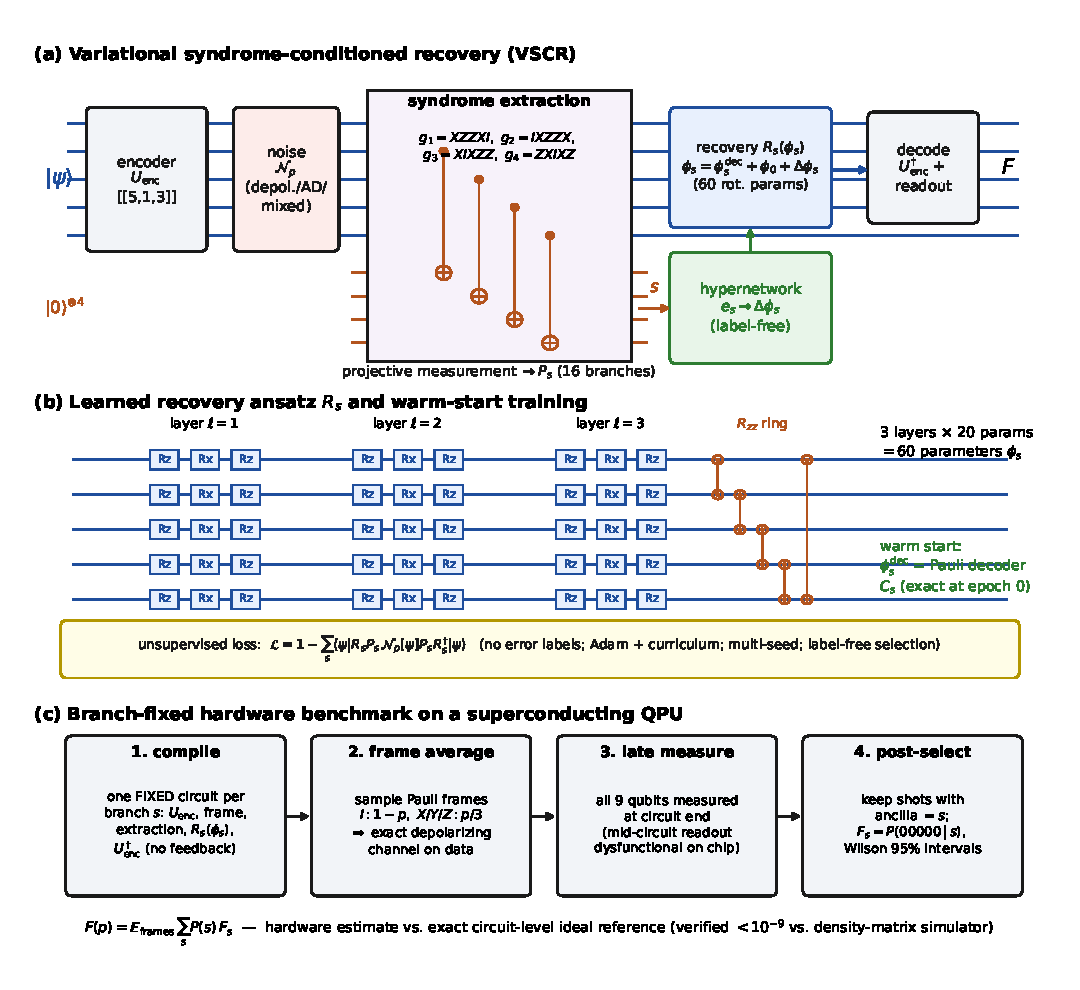
\includegraphics[width=\textwidth]{fig_schematic.pdf}
\caption{\textbf{VSCR 方法与硬件协议。}（a）该仪器：编码进 $\code$ 码、噪声、
到四个辅助比特上的投影式稳定子提取、由超网络条件化的学得恢复 $R_s$、解码与读出。
（b）恢复拟设与解码器热启动参数化。
（c）分支固定的硬件基准：编译、精确 Pauli 帧平均、后测、后选择。}
\label{fig:schematic}
\end{figure}

\begin{figure}[ht]
\centering
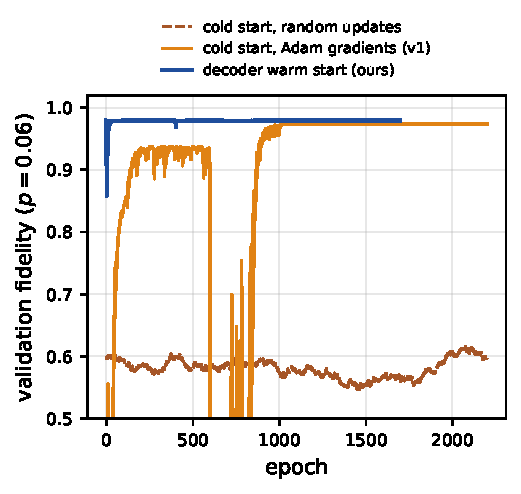
\includegraphics[width=0.55\textwidth]{fig_training.pdf}\\[4pt]
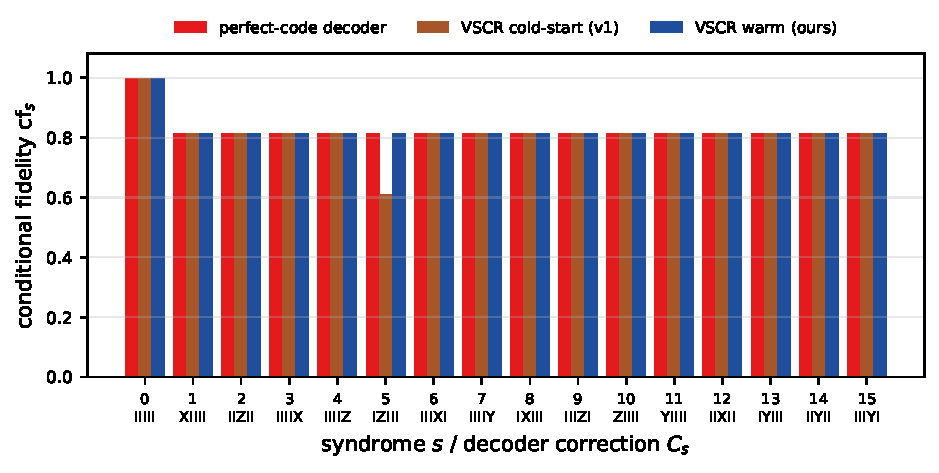
\includegraphics[width=\textwidth]{fig_branch_cf.pdf}
\caption{\textbf{训练与逐分支健康度。}（a）解码器热启动的 Adam 训练
对照冷启动训练与无梯度随机更新的验证保真度。（b）$p=0.15$（去极化）处
Pauli 解码器、冷启动模型与热启动模型的逐症候条件保真度 $\mathrm{cf}_s$：
热启动消除了冷启动变分恢复中不健康的分支，同时在每个分支上都达到解码器。}
\label{fig:training}
\end{figure}

\begin{figure}[ht]
\centering
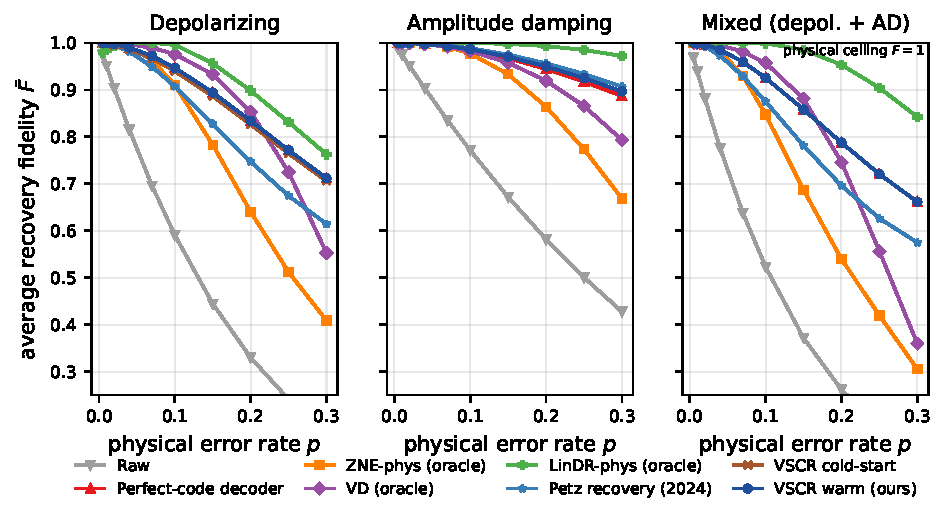
\includegraphics[width=\textwidth]{fig_sim_benchmark.pdf}\\[6pt]
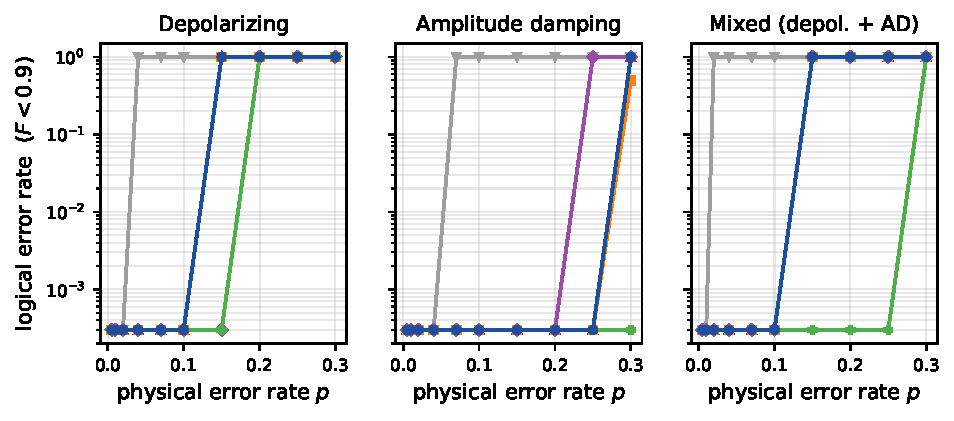
\includegraphics[width=\textwidth]{fig_sim_ler.pdf}\\[6pt]
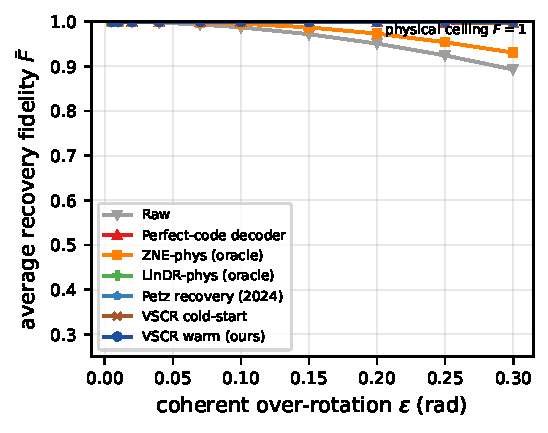
\includegraphics[width=0.62\textwidth]{fig_coherent.pdf}
\caption{\textbf{恢复基准。}去极化、振幅阻尼与混合噪声下平均保真度（上）
与逻辑错误率 $\Pr(F<0.9)$（中）随物理错误率的变化；相干过旋信道（下）。
误差带：$200$ 个随机逻辑态上的标准误差。每个方法都在一个\emph{物理}态上打分，
所以所有保真度轴都恰好封顶在 $1$ 处、并把物理上界 $\bar F=1$ 画成点线参考线，
评估对每个方法在每个噪声强度上都断言 $\bar F\le1+10^{-9}$。
零噪声外推以\emph{投影后}的形式报告（ZNE-phys）：原始 Richardson 估计量是外推算符的
一个无界线性泛函，在相干信道上对\emph{每一个}被审计的态、在\emph{每一个}强度上都超过 $1$
（在 $\varepsilon=0.30$ 处高达 $1.1306$），而在三个非相干信道上从不如此（$0/60$ 个态）；
因此一条未投影的 ZNE 曲线之所以会看起来赢得那个面板，纯粹是因为它离开了物理态空间
（见方法）。虚拟蒸馏在相干面板中被略去，因为那里 $\rho^2=\rho$
使它在代数上与 Raw 完全相同；这个恒等式被断言到机器精度（$1.6\times10^{-15}$），
而不是被画成一条重复的曲线。\emph{Petz 恢复（2024）}是式~\ref{eq:petz}
的噪声自适应恢复信道，用完全相同的估计量打分。
热启动的 VSCR 在去极化与混合噪声上与完美码解码器重合，
在那里解码器可证明是 CPTP 最优的（经认证提升空间 $\le10^{-15}$；ED 表~7），
而在振幅阻尼与相干噪声上\emph{高于}它与之分离——在 $p=0.10$ 的振幅阻尼上
$\bar F=0.98635$ 对照解码器的 $0.98475$，在 $\varepsilon=0.30$ 处
$\bar F=0.99997$ 对照 $0.99688$——在那里方法部分的可分离精化分别捕获了经认证非 Pauli
提升空间的 $90\%$ 与 $99.9996\%$。在所有情形下，解码器下界都在构造上保证
$\bar F_{\rm warm}\ge\bar F^{\rm dec}$。}
\label{fig:benchmark}
% 注意：相干过旋信道是这同一个浮动体的\emph{下面板}（上面的 fig_coherent.pdf），
% 而不是一个独立的图。因此它刻意没有自己的 `fig:coherent` 标签：
% 一个浮动体上的第二个标签会解析为同一个编号，从而读起来像一个悬空的自引用。
% 请把读者指向图~\ref{fig:benchmark} 并说“下面板”。
\end{figure}

\begin{figure}[ht]
\centering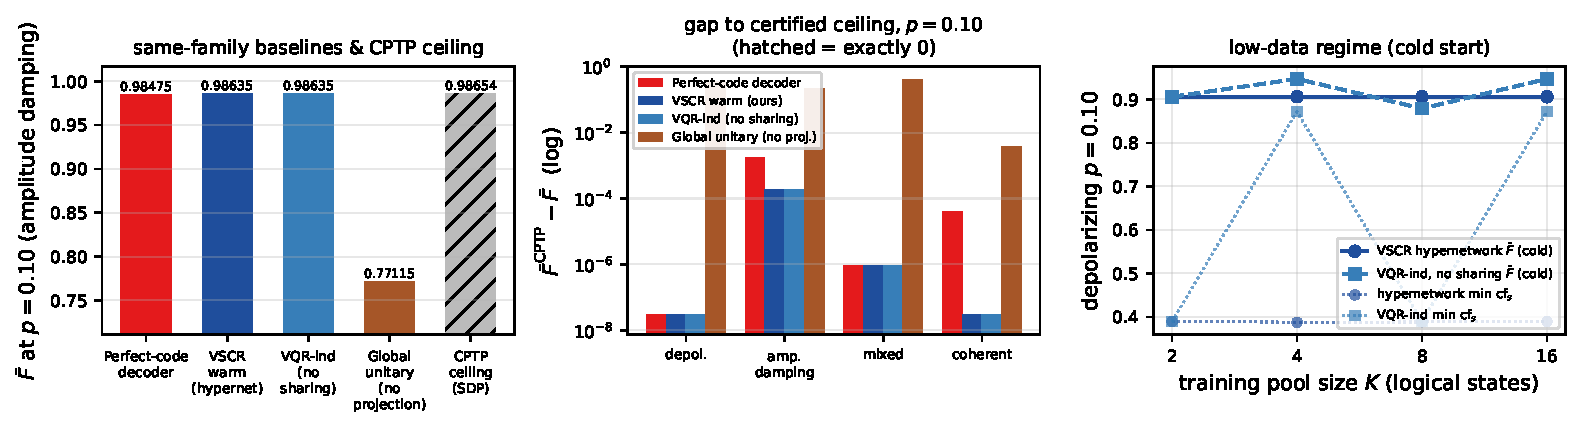
\includegraphics[width=\textwidth]{fig_ablation.pdf}
\caption{\textbf{同族基线、到经认证上界的差距，以及低数据消融。}
（a）$p=0.10$ 处的\emph{振幅阻尼}：完美码解码器、热启动 VSCR（超网络）、
VQR-ind（独立的逐症候角度表）、一个不做症候投影的全局变分幺正操作（QVECTOR 式），
以及 SDP 最优 CPTP 上界（阴影填充）。振幅阻尼是这些柱状条真正分离的那个信道
（上界比解码器高 $+1.8\times10^{-3}$，最差单分支高 $+0.195$）。
在去极化上，解码器、两种学得架构与上界反而相符到 $7\times10^{-12}$，
因为刚性 Pauli 解码器在那里\emph{精确}是 CPTP 最优的（ED 表~7）：
这是一个定理而不是一个空结果，但一个线性刻度的图表无法把它显示出来，
这正是面板（b）存在的原因。（b）到经认证上界的差距 $\bar F^{\rm CPTP}-\bar F$，
在对数刻度上给出全部四个信道的结果——这是唯一一种能使以下数值同时可读的呈现方式，
跨越八个数量级：精确的 $0$（去极化，那里每一种症候分辨方法都坐在上界上）、
$9\times10^{-7}$（混合）、解码器的 $1.8\times10^{-3}$ 对照 VSCR 的 $1.9\times10^{-4}$
（振幅阻尼）、$4.1\times10^{-5}$ 对照 $6.8\times10^{-9}$（相干，相差 $6000$ 倍），
以及 $4\times10^{-1}$（无投影的全局幺正操作）。（c）低数据区制：
在一个固定的 $K$ 个逻辑态池上做冷启动训练（去极化，在 $p=0.10$ 处用 $200$
个新态评估）；实线：平均保真度 $\bar F$，虚线：最差分支条件保真度
$\min_s\mathrm{cf}_s$。}
\label{fig:ablation}
\end{figure}
\begin{figure}[ht]
\centering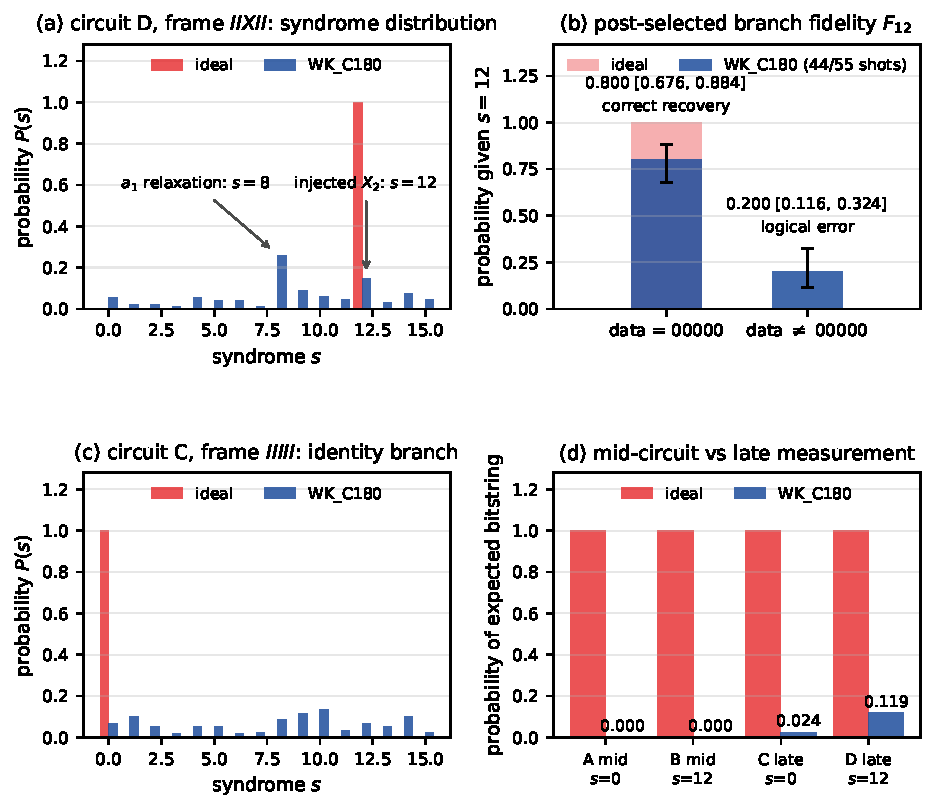
\includegraphics[width=\textwidth]{fig_hw_feasibility.pdf}
\caption{\textbf{OriginQ Wukong \texttt{WK\_C180} 上的硬件可行性。}
（a）注入 $X_2$（帧 $IIXII$）的后测电路的症候分布：$a_1$ 弛豫卫星峰 $s=8$
是众数，而正确读到的 $s=12$ 居第二，对照理想的 delta 分布。（b）后选择的恢复保真度
$F_{12}=0.80$（$44/55$ 次发射，Wilson $95\%$ 区间），对照理想值 $1.0$。
（c）恒等分支：硬件症候分布接近均匀。（d）每个电路中期望比特串的概率：
中测电路不产生信号；后测电路保留症候关联。}
\label{fig:hardware}
\end{figure}


\section*{数据可用性}

本文中的每一项定量论断都作为带版本的产物存储，并且可以从随附的开放仓库
\url{https://github.com/RichardYang88/QEC} 中的代码重新生成；
支撑本版本的快照将在投稿被接收时存入一个持久性档案库（Zenodo）并以 DOI 引用，
而那次存储即为数据的记录版本。
同一目录树中的 \texttt{paper/audit\_numbers.py} 从这些产物重新推导
稿件与扩展数据中引用的每一个数字，并在任何不一致处失败，
所以这些数据不仅是可获取的，而且是对照正文做过机器核验的。

\emph{仿真数据。}训练得到的角度集与逐分支条件保真度
（\texttt{vscr\_angles\_*.npz}、\texttt{vscr\_paper\_results.npz}、
\texttt{vscr\_paper\_abl\_results.npz}）；每个信道与强度下的平均保真度、
经认证上界与精化记录（\texttt{paper\_numbers.json}）；
精确的码尺寸标度扫描与读出律（\texttt{scaling\_results.json}）；
多种子统计（\texttt{multiseed\_results.json}）；
多轮存储与泄漏（\texttt{storage\_rounds.json}）。

\emph{证书数据。}九扇区驻点性证书及其 $90$ 对直接扫描
（\texttt{stationarity\_boundary.json}）；混合输入边界，
包括器件隐含的逻辑输入半径与它所定价的过度读出
（\texttt{mixed\_input\_boundary.json}）；Kraus 秩阶梯及其显式 Stinespring 膨胀
（\texttt{ancilla\_recovery.json}）。

\emph{硬件数据。}全部四个已执行电路的返回比特串计数及其派生的逐电路记录
（\texttt{hw\_feasibility\_numbers.json}），连同流水线写出的原始云端转储
（\texttt{qcloud\_raw\_*.json}、\texttt{qcloud\_results\_*.json}）；
有效误差预算、读出不对称性与精确门清单（\texttt{hw\_error\_budget.json}）；
编译后的分支电路及其精确理想参考值
（\texttt{paper\_numbers.json} 中的 \texttt{hardware\_frame\_numbers}）。

\emph{图与表的源数据。}图~1--5 的每一个面板与每一张扩展数据表，
都由仓库中的脚本从上述产物生成（\texttt{paper/make\_ed.py}、
\texttt{paper/fill\_numbers.py} 以及 \texttt{vscr\_paper*.py} 的绘图例程）；
没有任何一张图是从不在产物中的数字画出来的。

\emph{代码。}模拟器、训练流水线、证书脚本、硬件驱动与自检程序都在同一仓库中：
\texttt{ssvr\_qec.py}、\texttt{vscr\_general.py}、\texttt{vscr\_paper.py}、
\texttt{vscr\_paper\_coh.py}、\texttt{vscr\_paper\_abl.py}、
\texttt{scaling\_analysis.py}、\texttt{stationarity\_boundary.py}、
\texttt{mixed\_input\_boundary.py}、\texttt{ancilla\_recovery.py}、
\texttt{multiseed\_stats.py}、\texttt{storage\_rounds.py}、
\texttt{qcloud\_vscr\_new.py}、\texttt{hw\_verify\_analysis.py}、
\texttt{hw\_error\_budget.py} 与 \texttt{run\_selftests.py}。

\emph{限制。}有一类第三方数据不可获取，我们如实报告而不略去：
\texttt{WK\_C180} 的厂商校准（逐量子比特读出与单门保真度、$T_1$、$T_2$）
只在一次本账户已不再持有的授权之后暴露。那次拒绝连同其时间戳与错误字符串
被记录在 \texttt{hw\_error\_budget.json} 中；这也正是本文所引用的硬件误差预算
之所以是\emph{有效的}——即实测症候分布相对于一个确定性理想值的边缘量，
不含误差模型、不含拟合——而不是经校准的原因。
文献核验转储（\texttt{refs\_verification*.json}）一并纳入，
使每一条被引用的记录都可以逐字段重新核查。

\bibliography{refs}
\bibliographystyle{unsrtnat}

\end{document}

